\documentclass[letter,11pt]{article}
\usepackage{jheppub}
\usepackage{taro}
\usepackage{booktabs}

\newcommand{\red}[1]{\textcolor{red}{#1}}
\newcommand{\pink}[1]{\textcolor{pink}{#1}}
\newcommand{\blue}[1]{\textcolor{blue}{#1}}
\newcommand{\green}[1]{\textcolor{ForestGreen}{#1}}
\newcommand{\orange}[1]{\textcolor{orange}{#1}}
\newcommand{\brown}[1]{\textcolor{brown}{#1}}

\newcommand{\J}{\mathcal{J}}

\newcommand{\ab}[1]{\langle #1 \rangle}
\newcommand{\sqb}[1]{[ #1 ]}
\newcommand{\aMs}[3]{\langle #1|#2|#3]}  		% <1|2|3]
\newcommand{\aMMa}[3]{\langle #1|#2|#3\rangle}		% <1|Q_1.Q_2|3>
\newcommand{\sab}[1]{s_{#1}}
\newcommand{\twhite}[1]{\textcolor{white}{#1}}

\title{$N<4$ On-Shell Diagrams}

\def\Tr{{\rm Tr}}
\def\MHVbar{${\overline{\rm MHV}}$}
\def\nn{\nonumber}
\def\NeqFour{${\cal N}=4$}
\def\Split{{\rm Split}}
\def\spa#1.#2{\left\langle#1\,#2\right\rangle}
\def\spb#1.#2{\left[#1\,#2\right]}
\def\sandmx#1.#2.#3{%
	\left\langle#1{\vphantom1}\right|{#2}\left|#3\right]}%
\def\delt#1{\delta^{(#1)}}
\def\eps{\epsilon}
\def\Ord{{\cal O}}
\def\tlambda{\tilde\lambda}
\def\draftnote#1{{\sl #1}}
\def\tp{\!+\!}
\def\sA{{\cal A}}
\def\Int#1{I^{(#1)}}

\author[a]{Taro V. Brown}

\affiliation[a]{Department of Physics, UC Davis, One Shields Avenue, Davis, CA 95616, USA }


% e-mail addresses: one for each author, in the same order as the authors
\emailAdd{tvbrown@ucdavis.edu}


\abstract{Using on-shell diagrams we calculate various amplitudes in $\mathcal{N}=4$. We then extend this to $\mathcal{N}\neq4$ focusing on $\mathcal{N}=0$ and analyze the singularity structure of the results. Finally we calculate higher loop forms at five points.}

\begin{document} 
\maketitle
\flushbottom
\newpage
\section{Introduction}
During the last few decades, significant strides have been made in the study of scattering amplitudes. New modern on-shell techniques have made calculations with a large number of particles and loops feasible. Many of the significant advancements in the field has come by studying $\mathcal N = 4$ super Yang-Mills (sYM)
and using its planar, or large $N$, limit as a sandbox to explore the underlying geometric structure \cite{amp1,amp3,amp4,amp6,Elvang}.

In recent years this geometric structure of scattering amplitudes in $\mathcal N = 4$
sYM has been explored using the positive Grassmannian, on-shell diagrams, and
the Amplituhedron \cite{amp2,on1,on2}. A natural progression is to try and extend these discoveries beyond planar $\mathcal N = 4$ sYM to explore whether the geometric interpretation is a more general feature of quantum field theories (QFT’s). Similarly, considering theories with $\mathcal N\neq 4$, such as supergravity ($\mathcal N = 8$), will teach us to what extent these geometric pictures apply to other field theories. 

The focus of this project has been some of these extensions, with the report structured as follows. In section \ref{sec:grassmanian} we give a short review of the Grassmannian, followed by an introduction to on-shell diagrams. Then, in sections \ref{sec:on-she-intro} and \ref{sec:examples} we calculate various examples using the methods described. We extend this approach to theories for $\mathcal{N}\neq 4$ in section \ref{sec:YM}, focusing on $\mathcal N=0$ \footnote{The results found at $\mathcal{N}=0$ can easily be extended by adding super momentum delta functions in the calculation.}, explicitly calculating multiple examples at five and six points. Then diagrams at higher loops are considered in section \ref{sec:higherloops} and finally we consider the singularity structure of the results found.
\section{Grassmannian\label{sec:grassmanian}}
In this section we give a brief review of the Grassmannian, which will serve as a crucial ingredient for our discussion of on-shell diagrams.
The Grassmannian, denoted $G(k,n)$, is the space of $k$-planes going through the origin in $n$ dimensions. It can be thought of as a generalization of projective space $P^{n-1}$, which is the space of lines going through the origin in $n$-dimensions, since $G(1,n)=P^{n-1}$. One can e.g. take $k$ vectors in $n$ dimensions, see figure \ref{fig:1}
\begin{figure}[H]
	\centering
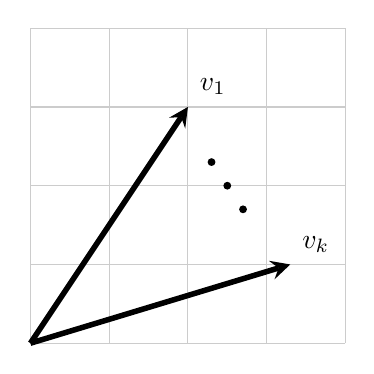
\begin{tikzpicture}{scale=0.5}
	\draw[thin,gray!40] (0,0) grid (4,4);
	\draw[line width=2pt,black,-stealth](0,0)--(2,3) node[anchor=south west]{$\boldsymbol{v_1}$};
	\node at (2.3,2.3) [circle,fill,inner sep=1pt]{};
	\node at (2.5,2.0) [circle,fill,inner sep=1pt]{};
	\node at (2.7,1.7) [circle,fill,inner sep=1pt]{};
	\draw[line width=2pt,black,-stealth](0,0)--(3.3,1) node[anchor=south west]{$\boldsymbol{v_k}$};
\end{tikzpicture}
\label{fig:1}
\caption{$k$ $n$-dimensional vectors going through the origin}
\end{figure}
The span of these vectors gives the $k$- plane. If they are stacked, we get a matrix $C_{\alpha a}$
\begin{equation}
\begin{aligned}
	&~~~~~~~n\\
	k&
\begin{bmatrix}
	~~~~V_1~~~~~\\
	~~~~\vdots ~~~~~\\
	~~~~V_k~~~~~\\
\end{bmatrix}\equiv C_{\alpha a},~~~~~~~~\alpha=1,\dots,k~~~~a=1,\dots,n
\end{aligned}
\end{equation}
This matrix is generally not unique since it has a GL($k$) redundancy, $
C_{\alpha a}\sim L^{\beta}_\alpha C_{\beta a}$.
The dimensionality of the Grassmannian is 
\begin{equation}
\dim G(k,n)=\overbrace{k\times n}^{k\times n \text{ matrix}}\underbrace{-k^2}_{GL(k) \text{ red}}
\end{equation}
The redudancy means that we can gaugefix the matrix using a linear transformation by setting any $k\times k$ blok to the identity. This is equivalent to the rescaling of a vector in projective space to $\begin{pmatrix}
1 & v_2 & v_3 & v_4 \cdots
\end{pmatrix}$. Taking e.g. $G(3,5)$, we have six degrees of freedom:
\begin{equation}G(3,5) = 
\left[ \begin{array}{@{}c|c@{}}
	\begin{matrix}
		1 & 0 &  0 \\
		0 & 1 &  0 \\
		0 & 0 &  1 \\
	\end{matrix} 
	& 	\begin{matrix}
		x_4 & x_5  \\
		y_4 & y_5  \\
		z_4 & z_5  \\
	\end{matrix}  \\
\end{array} \right]
\end{equation}
The dimensionality of the Grassmannian is symmetric under $n\leftrightarrow k$. This is because there is a bijection between the Grassmania: $k$ and $n-k$ planes in $n$ dimensions, since these planes are orthogonal. In the case above $C^{\perp}$ is a $2$-plane in 5 dimensions. We can illustrate both the matrices like so,
\begin{equation}
	\left[ \begin{array}{@{}c|c@{}}
		\begin{matrix}
			1 & 0 &  0 \\
			0 & 1 &  0 \\
			0 & 0 &  1 \\
		\end{matrix} 
		& 	\begin{matrix}
			x_4 & x_5  \\
			y_4 & y_5  \\
			z_4 & z_5  \\
		\end{matrix}  \\
	\cmidrule[0.4pt]{1-2}
		\begin{matrix}
		-x_4 & -y_4 & -z_4  \\
		-x_5 & -y_5 & -z_5 \\
	\end{matrix} 
	& 	\begin{matrix}
	1 & 0  \\
	0 & 1  \\
\end{matrix} 
	\end{array} \right]
\end{equation}
With the bottom part just being the negative transpose of the $x,y$ and $z$ coordinates in the upper right corner. The invariants are determinants of any $k$ minors, labeling these by their indices:
\begin{equation}
\begin{pmatrix}
a_1&a_2&\cdots &a_k
\end{pmatrix}
\end{equation}
We will now proceed to use the properties of the Grassmannian by introducing the concept of on-shell diagrams.
\newpage
\section{Introduction to on-shell diagrams}\label{sec:on-she-intro}
In this section we introduce the notion of on-shell diagrams, and give examples on different ways one can calculate differential forms from these. 

One can construct $(k\times n)$ C-matrices out of on-shell diagrams, where $k$ labels the number of negative helicity particles and $n$ is the total number of particles. The procedure to construct a matrix from a diagram using \textit{edge-variables} is as follows
\begin{itemize}
	\item Label the edges of the on-shell diagram by $\alpha$'s. Not all edges have to be labeled due to the GL$(k)$ redundancy.
	\item Starting at one of the incoming particles (say, $2$), trace a path to one of the outgoing particles  (say, $4$). Multiply the $\alpha$'s encountered on the path. This would be entry $C_{2\,4}$ in the C-matrix, i.e.
	\begin{equation}
		\begin{aligned}
			C_{ab}=\sum_{\Gamma(a\to b)}\prod_j\alpha_j
		\end{aligned}
	\end{equation}
	\item When going from an incoming particle to another incoming particle, put a $0$ in that matrix entry, unless it is a path starting and ending at the same particle, then put a $1$.
	\item If the path encounters an internal cycle that forms a complete loop, the matrix element is multiplied by the geometric series, labeled by $\delta$, containing the edge-variables encountered in that loop, i.e.
	\begin{equation}
		\begin{aligned}
			\delta=\sum_{n=0}^\infty (\alpha_i \alpha_j\alpha_k \cdots)^n=\frac{1}{1- (\alpha_i \alpha_j\alpha_k \cdots)}
		\end{aligned}
	\end{equation}
	\item The form is then found through
	\begin{equation}
		\begin{aligned}
			\dd \Omega =\prod_{i=1}^{N}\frac{\dd \alpha_i}{\alpha_i}\delta(C\cdot Z)\mathcal{J}^{\mathcal{N}-4}
		\end{aligned}
	\end{equation}
\end{itemize} 
where $\delta(C\cdot Z)\equiv\delta(C\cdot \tilde \lambda) \delta(C^\perp\cdot \lambda)\delta(C\cdot \tilde \eta)$, and $\mathcal{J}$ is a Jacobian which we will describe in further detail in section \ref{sec:YM}.
We will now calculate amplitudes through various techniques using the on-shell diagrams. 
\subsection{Three point on-shell form} 
The easiest example is the two diagrams representing the three-point MHV and $\overline{\text{MHV}}$ amplitudes in $\mathcal{N}=4$ sYM.
Taking e.g the amplitudes to be $A_3^{\text{MHV}}(1^-,2^-,3^+)$ and $A_3^{\overline{\text{MHV}}}(1^+,2^+,3^-)$, the on-shell diagrams are\\
\begin{figure}[H]\centering\hspace*{1.5cm}
	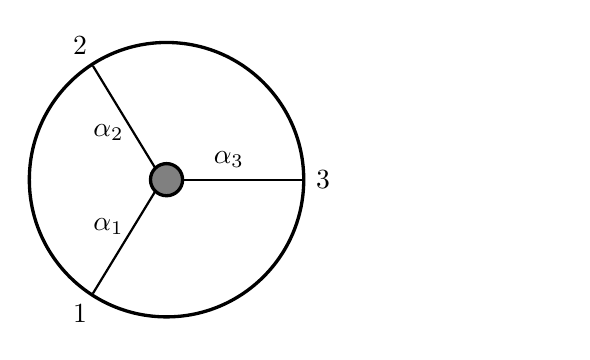
\begin{tikzpicture}[scale=0.85]
		\begin{scope}[very thick, every node/.style={sloped,allow upside down}]
			\draw[black,fill=gray] (0,0) circle (2.4mm);
			\draw (0,0) circle (20.5mm);
			\draw[thick,black] (-1.1,1.7) -- node {\midarrow} (-0.16,0.16);
			\draw[thick,black] (-1.1,-1.7) -- node {\midarrow} (-0.16,-0.16);
			\draw[thick,black] (0.24,0) -- node {\midarrow} (2.05,0);
			\node[text width=0.5cm] at (-1.1,2.0) {2};
			\node[text width=0.5cm] at (-1.1,-2.0) {1};
			\node[text width=3cm] at (4,0) {3};
				\node[text width=0.5cm] at (-0.8,-0.7) {$\alpha_1$};
				\node[text width=0.5cm] at (-0.8,0.7) {$\alpha_2$};
				\node[text width=0.5cm] at (1,0.3) {$\alpha_3$};
		\end{scope}
	\end{tikzpicture}
	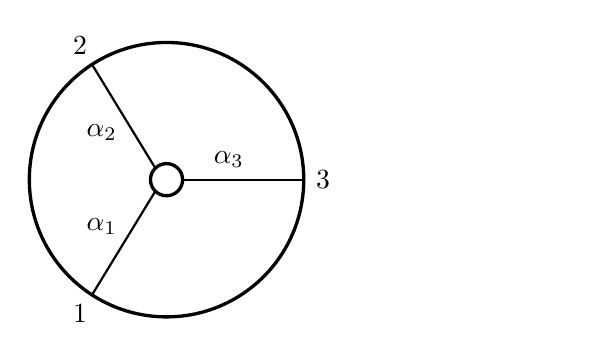
\begin{tikzpicture}[scale=0.85]
	\begin{scope}[very thick, every node/.style={sloped,allow upside down}]
		\draw[black] (0,0) circle (2.4mm);
		\draw (0,0) circle (20.5mm);
		\draw[thick,black] (-0.16,0.16) -- node {\midarrow} (-1.1,1.7);
		\draw[thick,black] (-0.16,-0.16) -- node {\midarrow} (-1.1,-1.7);
		\draw[thick,black] (2.05,0) -- node {\midarrow} (0.24,0);
		\node[text width=0.5cm] at (-1.1,2.0) {2};
		\node[text width=0.5cm] at (-1.1,-2.0) {1};
		\node[text width=3cm] at (4,0) {3};
		\node[text width=0.5cm] at (-0.9,-0.7) {$\alpha_1$};
		\node[text width=0.5cm] at (-0.9,0.7) {$\alpha_2$};
		\node[text width=0.5cm] at (1,0.3) {$\alpha_3$};
	\end{scope}
\end{tikzpicture}
\end{figure}
\noindent
These produce the two following $C$ matrices, respectively
\begin{equation}
	\begin{aligned}
		C&=\begin{pmatrix}
			1 & 0 & \alpha_1\alpha_2 \\ 0 & 1 & \alpha_2\alpha_3
		\end{pmatrix},~~~~~~~~~~~~C=\begin{pmatrix}
		\alpha_1\alpha_3 & \alpha_2\alpha_3 & 1
	\end{pmatrix}
	\end{aligned}
\end{equation}
The amplitudes in this case are
\begin{equation}
	\begin{aligned}
		A_3^{\text{MHV}}(1,2,3)&=\frac{\delta\left(\mathcal Q\right)\delta\left(P\right)}{\expval{12}\expval{23}\expval{31}}\\
		A_3^{\overline{\text{MHV}}}(1,2,3)&=\frac{\delta\left([12]\tilde\eta_3+[23]\tilde\eta_1+[31]\tilde\eta_2\right)\delta\left(P\right)}{[12][23][31]}\\
	\end{aligned}
\end{equation}
where $\mathcal Q\equiv \sum_{i=1}^{3}\lambda_i\tilde\eta_i$ and $P\equiv \sum_{i=1}^{3}\lambda_i\tilde\lambda_i$
One can further construct more elaborate diagrams by gluing these three point functions together.
The simplest possible diagram, found by stitching together two vertices of opposite helicity ($k=1$ and $k=2$), is shown below
\begin{figure}[H]\centering\hspace*{3cm}
	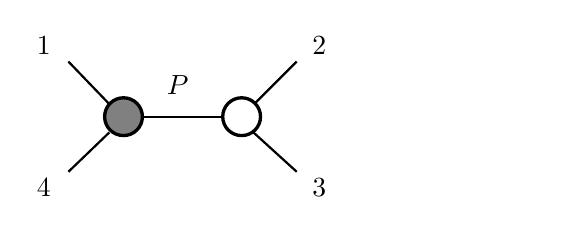
\begin{tikzpicture}
		\begin{scope}[very thick, every node/.style={sloped,allow upside down}]
			\draw (1.5,1.5) circle (2.4mm);
			\draw[black,fill=gray] (0,1.5) circle (2.4mm);
			\draw[thick,black] (0.25,1.5) -- node {\midarrow} (1.25,1.5);
			\node[text width=0.5cm] at (0.8,1.9) {$P$};
			\draw[thick,black] (-0.18,1.3) --  (-0.7,0.8); %4
			\draw[thick,black] (1.67,1.67) --   (2.2,2.2);
			\draw[thick,black] (-0.7,2.2) -- (-0.19,1.67);
			\draw[thick,black] (2.2,0.8) -- (1.65,1.3); %3
			\node[text width=3cm] at (0.4,2.4) {1};
			\node[text width=3cm] at (3.9,2.4) {2};
			\node[text width=3cm] at (3.9,0.6) {3};
			\node[text width=3cm] at (0.4,0.6) {4};
		\end{scope}
	\end{tikzpicture}
\end{figure}
\noindent To construct the four-point diagram we then glue the two three-point amplitudes together by integrating over the internal degrees of freedom through
\begin{equation}
	\begin{aligned}
		\prod_{I}\int \dd^4 \tilde \eta_I \int\frac{d^2\lambda_Id^2\tilde\lambda_I}{GL(1)}
	\end{aligned}
\end{equation}
Explicitly we have
\begin{equation}
	\begin{aligned}
		\int \dd \tilde \eta_{P} \int\frac{d^2\lambda_Pd^2\tilde\lambda_P}{GL(1)}&
		\frac{\delta^{8}\left(\lambda_1\tilde\eta_1+\lambda_{4}\tilde\eta_{4}+\lambda_{P}\tilde\eta_{P}\right)\delta^{4}\left(\lambda_{1}\tilde\lambda_{1}+\lambda_{4}\tilde\lambda_{4}+\lambda_{P}\tilde\lambda_{P}\right)}{\expval{14}\expval{4P}\expval{P1}}\\
		\times&\frac{\delta^{4}\left([23]\tilde\eta_{P}+[3P]\tilde\eta_{2}+[P 3]\tilde\eta_{3}\right)\delta^{4}\left(\lambda_{2}\tilde\lambda_{2}+\lambda_{3}\tilde\lambda_{3}-\lambda_{P}\tilde\lambda_{P}
			\right)}{[23][3P][P2]}
	\end{aligned}
\end{equation}
First we solve the delta-function constraint by projecting along $\lambda_1$
\begin{equation}
	\begin{aligned}
		&\lambda_{1}\tilde\lambda_{1}+\lambda_{4}\tilde\lambda_{4}+\lambda_{P}\tilde\lambda_{P}=0\\
		\Rightarrow& \tilde\lambda_{P}=\frac{\expval{41}}{\expval{1P}}\tilde\lambda_4.
	\end{aligned}
\end{equation}
Similarly we use the other delta-function and project using $\tilde \lambda_3$
\begin{equation}
	\begin{aligned}
		&\lambda_{2}\tilde\lambda_{2}+\lambda_{3}\tilde\lambda_{3}-\lambda_{P}\tilde\lambda_{P}=0\\
		\Rightarrow& 
		\lambda_{P}=\frac{[23]}{[P3]}\lambda_2.
	\end{aligned}
\end{equation}
Combining these we obtain
\begin{equation}
	\begin{aligned}
		\tilde\lambda_P \lambda_P=\lambda_2 \tilde\lambda_4 \frac{\expval{41}[23]}{\expval{1P}[P3]}&=\lambda_2 \tilde\lambda_4 \frac{[23]}{[43]}\\
		&=\lambda_2 \tilde\lambda_4 \frac{\expval{41}}{\expval{12}}
 	\end{aligned}
\end{equation}
where we have used $P=-1-4=2+3$ in the last two equalities. Solving this collapses the momentum conservation delta function as well as giving a Jacobian factor of $\frac{1}{\expval{23}[32]}$
\begin{equation} \label{eq:sol3}
	\begin{aligned}
		\lambda_P&=\lambda_2\\
		\tilde \lambda_P&=\lambda_4 \frac{\expval{41}}{\expval{12}}=\tilde\lambda_4 \frac{[23]}{[43]}
	\end{aligned}
\end{equation}
We then use these in one of the grassmann delta-functions
\begin{equation}
	\begin{aligned}
		\tilde\eta_{P}&=\frac{-[3P]\tilde\eta_{2}-[P 2]\tilde\eta_{3}}{[23]}\\
		&=-\frac{1}{[23]}\times \frac{[34][23]}{[43]} \times\tilde \eta_2-\frac{1}{[23]}\times \frac{[42]\expval{41}}{\expval{12}} \times\tilde \eta_3\\
		&=\tilde \eta_2+ \frac{\expval{13}}{\expval{12}} \times\tilde \eta_3\\
	\end{aligned}
\end{equation}
This can be obtained from contracting
\begin{equation}
	\begin{aligned}
\lambda_P\tilde\eta_{P}	&=\lambda_2\tilde \eta_2+ \lambda_3 \tilde \eta_3\\	
	\end{aligned}
\end{equation}
 with $\lambda_1$, since $\lambda_P=\lambda_2$. Using this in the other grassmann  delta function we get $[23]^4\delta^8(\sum_i\lambda_i\tilde\eta_i)$. Finally we take the solutions \eqref{eq:sol3} and insert them into the bosonic delta-function
 \begin{equation}
 	\begin{aligned}
 		0&=\lambda_1\tilde\lambda_1+\lambda_4\tilde\lambda_4+\lambda_P\tilde\lambda_P
 		=\lambda_1\tilde\lambda_1+\tilde\lambda_4 \left(\lambda_4+\lambda_2  \frac{[23]}{[43]}\right)
 		\\
 		&=\lambda_1\tilde\lambda_1+\tilde\lambda_4 \left(  \frac{\lambda_4[43]+\lambda_2[23]}{[43]}\right)=\lambda_1 \left(\tilde\lambda_1 +\tilde\lambda_4 \frac{[13]}{[34]}\right)
 			\\
 		&=\lambda_1 \left( \frac{\tilde\lambda_1[34]+\tilde\lambda_4[13]}{[34]}\right)=\lambda_1 \tilde\lambda_3 \frac{[14]}{[34]}
 	\end{aligned}
 \end{equation}
Since $\lambda_1\neq0,$ and $\tilde\lambda_3\neq0$ this leads to $[14]=0$ which in turn gives us
\begin{equation}
	\begin{aligned}
		(p_1+p_4)^2=\expval{14}[41]=0
	\end{aligned}
\end{equation}
Now we only need the kinematic part of the integrand. Including the Jacobians and using $\expval{1P}[P3]=\expval{12}[23]$ and $\expval{4P}[P2]=\expval{43}[32]$ we obtain
\begin{equation}
	\begin{aligned}
		\frac{1}{\expval{14}\expval{4P}\expval{P1}}\times\frac{1}{[23][3P][P2]}\times \frac{[23]^4}{\expval{23}[23]}&=\frac{1}{\expval{12}\expval{23}\expval{34}\expval{41}}\\
	\end{aligned}
\end{equation}
Such that we in total have the form
\begin{equation}
	\begin{aligned}
		\frac{\delta^{8}\left(\mathcal{Q}\right)\delta^{4}\left(P\right)}{\expval{12}\expval{23}\expval{34}\expval{41}}\delta((p_1+p_4)^2)
	\end{aligned}
\end{equation}
This is not surprising since the diagram we considered is not a Feynman diagram. Rather the first diagram to give the four-point on-shell amplitude arises from gluing 4 three-point functions together
\begin{figure}[H]\centering \hspace*{3cm}
	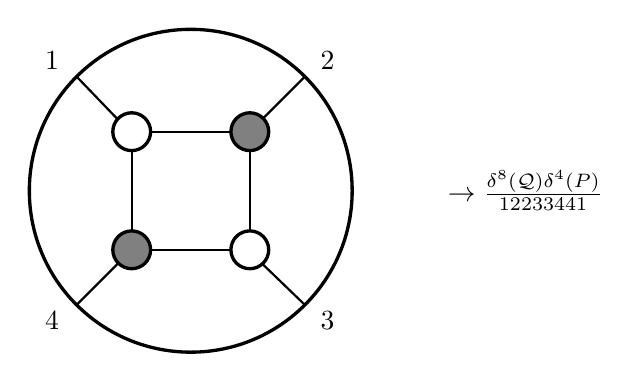
\begin{tikzpicture}
		\begin{scope}[very thick, every node/.style={sloped,allow upside down}]
			\draw[black,fill=gray] (0,0) circle (2.4mm);
			\draw (1.5,0) circle (2.4mm);
			\draw[black,fill=gray] (1.5,1.5) circle (2.4mm);
			\draw (0,1.5) circle (2.4mm);
			\draw[thick,black] (1.25,0) -- node {\midarrow} (0.25,0);
			\draw[thick,black] (0.25,1.5) -- node {\midarrow} (1.25,1.5);
			\draw[thick,black] (0,1.25) -- node {\midarrow} (0,0.25);
			\draw[thick,black] (1.5,1.25) -- node {\midarrow} (1.5,0.25);
			\draw[thick,black] (-0.18,-0.18) -- node {\midarrow} (-0.7,-0.7);
			\draw[thick,black] (2.2,2.2) --  node {\midarrow}  (1.67,1.67) ;
			\draw[thick,black] (-0.7,2.2) -- node {\midarrow} (-0.19,1.67);
			\draw[thick,black] (1.65,-0.17) -- node {\midarrow} (2.2,-0.7);
			\draw (0.75,0.75) circle (20.5mm);
			\node[text width=3cm] at (0.4,2.4) {1};
			\node[text width=3cm] at (3.9,2.4) {2};
			\node[text width=3cm] at (3.9,-0.9) {3};
			\node[text width=3cm] at (0.4,-0.9) {4};
		\end{scope}
	\node at (5,0.75) {$\rightarrow\frac{\delta^{8}\left(\mathcal{Q}\right)\delta^{4}\left(P\right)}{\expval{12}\expval{23}\expval{34}\expval{41}}$};
	\end{tikzpicture}
\end{figure}
In the next section we will present two methods of getting the amplitude directly from the diagram.
\subsection{Four-point directly from $G(2,4)$ matrix}
The calculation of the $C$-matrix can be performed either using face or edge variables. We are going to show how to do both for good measure.
\subsubsection{Using face-variables}
The four-point diagram with face-variables looks like this
%%%%%%%%%%%%%%%%%%%%%%%%%%%%%%%%%%%%%%%%%%%%%%%%%%%%%%%%%%%%%%%%%%%%%%%%
\begin{figure}[H]\centering \hspace*{3cm}
	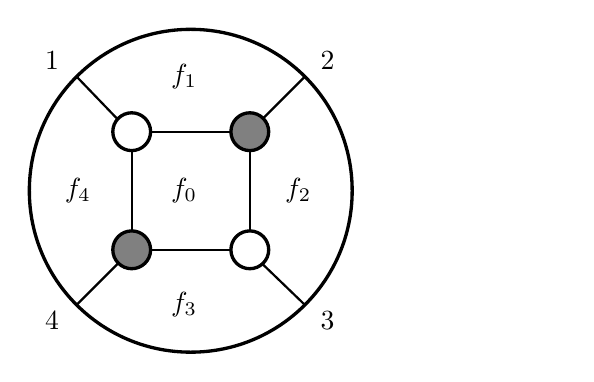
\begin{tikzpicture}
		\begin{scope}[very thick, every node/.style={sloped,allow upside down}]
			\draw[black,fill=gray] (0,0) circle (2.4mm);
			\draw (1.5,0) circle (2.4mm);
			\draw[black,fill=gray] (1.5,1.5) circle (2.4mm);
			\draw (0,1.5) circle (2.4mm);
			\draw[thick,black] (1.25,0) -- node {\midarrow} (0.25,0);
			\node[text width=0.5cm] at (0.75,-0.7) {$f_3$};
			\draw[thick,black] (0.25,1.5) -- node {\midarrow} (1.25,1.5);
			\node[text width=0.5cm] at (0.75,2.2) {$f_1$};
			\draw[thick,black] (0,1.25) -- node {\midarrow} (0,0.25);
			\node[text width=0.5cm] at (-0.6,0.75) {$f_4$};
			\draw[thick,black] (1.5,1.25) -- node {\midarrow} (1.5,0.25);
			\node[text width=0.5cm] at (2.2,0.75) {$f_2$};
			\node[text width=0.5cm] at (0.75,0.75) {$f_0$};
			\draw[thick,black] (-0.18,-0.18) -- node {\midarrow} (-0.7,-0.7);
			\draw[thick,black] (2.2,2.2) --  node {\midarrow}  (1.67,1.67) ;
			\draw[thick,black] (-0.7,2.2) -- node {\midarrow} (-0.19,1.67);
			\draw[thick,black] (1.65,-0.17) -- node {\midarrow} (2.2,-0.7);
			\draw (0.75,0.75) circle (20.5mm);
			\node[text width=3cm] at (0.4,2.4) {1};
			\node[text width=3cm] at (3.9,2.4) {2};
			\node[text width=3cm] at (3.9,-0.9) {3};
			\node[text width=3cm] at (0.4,-0.9) {4};
		\end{scope}
	\end{tikzpicture}
\end{figure}
\noindent While the $C$-matrix is found through
\begin{equation}
	\begin{aligned}
		C_{ab}=-\sum_{\Gamma(a\to b)}\prod_j\left(-f_j\right),~~~~~~\text{ on the right} 
	\end{aligned}
\end{equation}
with the added constraint
\begin{equation}
	\begin{aligned} \label{eq:prodf}
		\prod_j f_j=-1
	\end{aligned}
\end{equation}
%%%%%%%%%%%%%%%%%%%%%%%%%%%%%%%%%%%%%%%%%%%%%%%%%%%%%%%%%%%%%%%%%%%%%%%%%%%%%%%%%%%%%%%%%%%%%%%%%%%%%%%%%%%%%%%%%%%%%%%%%%%%%%%
Using the above, we find the matrix to have the following entries
\begin{equation}
	\begin{aligned}
		C=
		\begin{pmatrix}
			1 & 0 & f_0f_3f_4 & f_4(1-f_0)\\
			0 & 1 & -f_0f_1f_3f_4&f_0f_1f_4
		\end{pmatrix}
	\end{aligned}
\end{equation}
Note that $f_2$ doesn't appear, which means that according to \eqref{eq:prodf} we can take the remaining $f$'s as independent. Positivity (all minors are positive) then demands that
\begin{equation}
	\begin{aligned}
		f_0<0,~~~~f_1>0,~~~~f_2<0,~~~~f_3<0,~~~~
	\end{aligned}
\end{equation}
While the perpendicular C-matrix satisfying $C\cdot C^\perp=0$ is easily obtained
\begin{equation}
	\begin{aligned}
		C^\perp=
		\begin{pmatrix}
		 -f_0f_3f_4 &f_0f_1f_3f_4 & 1 & 0\\
		-f_4(1-f_0) &-f_0f_1f_4 & 0 & 1
		\end{pmatrix}
	\end{aligned}
\end{equation}
we can then find the form through
\begin{equation}
	\begin{aligned}
		\dd \Omega =\frac{\dd f_0}{f_0}\frac{\dd f_1}{f_1}\frac{\dd f_3}{f_3}\frac{\dd f_4}{f_4}\delta(C\cdot \tilde \lambda) \delta(C^\perp\cdot \lambda)\delta(C\cdot \tilde \eta)
	\end{aligned}
\end{equation}
First let us look at the delta-functions, such that we can specify the face-variables in terms of the spinor products. We start by looking at $\lambda \cdot C^\perp=0$, from which we get two equations
\begin{equation}
	\begin{aligned}
		C^\perp\cdot \lambda=0\Rightarrow\begin{cases}
			-\lambda_1f_0f_3f_4+\lambda_2 f_0f_1f_3f_4+ \lambda_3&=0\\
			-\lambda_1f_4(1-f_0)-\lambda_2f_0f_1f_4+ \lambda_4&=0
		\end{cases}
	\end{aligned}
\end{equation}
By multiplying the first equation by $ \lambda_2$ one obtains $f_0f_3f_4=-\frac{\expval{23}}{\expval{12}}$. Similarly multiplying the second equation by $ \lambda_1$ we get $f_0f_1f_4= \frac{\expval{14}}{\expval{12}}$. Combining these two,
\begin{equation}
	\begin{aligned}
		f_1=-\frac{\expval{14}}{\expval{23}}f_3
	\end{aligned}
\end{equation}
Then multiplying the first equation by $\tilde\lambda_1$ we have $f_0f_1f_3f_4=-\frac{\expval{13}}{\expval{12}}$ together with the previous result, this leads to
\begin{equation}
	\begin{aligned}
		f_3 =-\frac{\expval{13}}{\expval{14}} ~~~~~\text{and }~~~~~f_1 =\frac{\expval{13}}{\expval{23}} 
	\end{aligned}
\end{equation}
The other equations are solved similarly and we obtain
\begin{equation}
	\begin{aligned}
		f_0=&-\frac{\expval{14}\expval{23}}{\expval{12}\expval{34}}\\
		f_4=&-\frac{\expval{34}}{\expval{13}} 
	\end{aligned}
\end{equation}
%%%%%%%%%%%%%%%%%%%%%%%%%%%%%%%%%%%%%%%%%%%%%%%%%%%%%%%%%%%%%%%%%%%%%%%%
Let us now evaluate the two remaining delta-functions. From $C\cdot \tilde \lambda$ we get two equations. 
\begin{equation}
	\begin{aligned}
		0=\tilde\lambda_1+f_0f_3f_4 \tilde\lambda_3+f_4(1-f_0)\tilde\lambda_4=\tilde\lambda_1+\frac{\expval{32}}{\expval{12}} \tilde\lambda_3+\frac{\expval{42}}{\expval{12}} \tilde\lambda_4
	\end{aligned}
\end{equation}
and
\begin{equation}
	\begin{aligned}
		0=\tilde\lambda_2+\frac{\expval{13}}{\expval{12}} \tilde\lambda_3+\frac{\expval{14}}{\expval{12}} \tilde\lambda_4
	\end{aligned}
\end{equation}
where we have used a Schouten identity for the coefficient of $\tilde\lambda_4$
\begin{equation}
	\begin{aligned}
		\expval{41}\expval{23}+\expval{12}\expval{34}=\expval{13}\expval{24}
	\end{aligned}
\end{equation}
We see that these equations can all be obtained from a momentum conservation delta-function by contracting it with $\lambda_1$ and $\lambda_2$
\begin{equation}
\begin{aligned}
	\delta^{4}(\lambda_1\tilde\lambda_1+\lambda_2\tilde\lambda_2+\lambda_3\tilde\lambda_3+\lambda_4\tilde\lambda_4)\equiv \delta^{4}\left(P\right)
\end{aligned}
\end{equation}
For the last delta-function we get the exact same thing except for replacing $\tilde \lambda_i\to \tilde \eta_i$
\begin{equation}
\begin{aligned}
	\delta^{8}(\lambda_1\tilde\eta_1+\lambda_2\tilde\eta_2+\lambda_3\tilde\eta_3+\lambda_4\tilde\eta_4)\equiv \delta^{8}\left(\mathcal{Q}\right)
\end{aligned}
\end{equation}
Note that we get an extra factor of $\frac{1}{\expval{12}^4}$ from re-writing the delta-functions by projecting along $\lambda_1$ and $\lambda_2$. Finally we get a Jacobian from solving the delta-function constraints
\begin{equation}
	\begin{aligned}
		J=\left|J_{ij}\right|=f_0^2f_1f_3f_4^3=\frac{\expval{23}\expval{34}\expval{41}}{\expval{12}^2\expval{13}}
	\end{aligned}
\end{equation}
where
\begin{equation}
	\begin{aligned}
		J_{ij}=\pdv{E_i}{f_j}=\begin{pmatrix}
			f_3f_3 & 0 & f_0f_3 & f_0f_4\\
			f_1f_3f_4 &f_0f_3f_4 &f_0f_1f_4 & f_0f_1f_3\\
			f_4 & 0 & 0 & 1-f_0\\
			f_1f_4 & f_0f_4 & 0 & f_0f_1
		\end{pmatrix}
	\end{aligned}
\end{equation}
and 
\begin{equation}
	\begin{aligned}
		E_1=f_0f_3f_4,~~~~E_2=f_0f_1f_3f_4,~~~~E_3=f_4(1-f_0),~~~~E_4=f_0f_1f_3
	\end{aligned}
\end{equation}
Now using
\begin{equation}
	\begin{aligned}
		f_0f_1f_3f_4=\frac{\expval{13}}{\expval{12}}
	\end{aligned}
\end{equation}
We can put it all together to obtain the form
\begin{equation}
	\begin{aligned}
		\dd \Omega =\frac{\expval{12}}{\expval{13}}\times \frac{\expval{12}^2\expval{13}}{
			\expval{23}\expval{34}\expval{41}}\times \frac{1}{\expval{12}^4}\times \delta^4(P)\delta^8(\mathcal{Q})=\frac{\delta^{8}\left(\mathcal{Q}\right)\delta^{4}\left(P\right)}{\expval{12}\expval{23}\expval{34}\expval{41}}
	\end{aligned}
\end{equation}
%%%%%%%%%%%%%%%%%%%%%%%%%%%%%%%%%%%%%%%%%%%%%%%%%%%%%%%%%%%%%%%%%%%%%%%%
\subsubsection{Using edge-variables}
For the remainder of the report we will use instead be using edge-variables in the $C$-matrices.
To demonstrate how this approach works, we look at a diagram with a different orientation,
\begin{figure}[H]\centering\hspace*{3cm}
	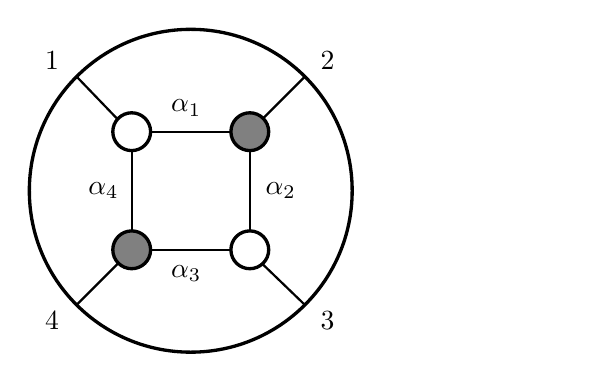
\begin{tikzpicture}
		\begin{scope}[very thick, every node/.style={sloped,allow upside down}]
			\draw[black,fill=gray] (0,0) circle (2.4mm);
			\draw (1.5,0) circle (2.4mm);
			\draw[black,fill=gray] (1.5,1.5) circle (2.4mm);
			\draw (0,1.5) circle (2.4mm);
			\draw[thick,black] (1.25,0) -- node {\midarrow} (0.25,0);
			\node[text width=0.5cm] at (0.75,-0.3) {$\alpha_3$};
			\draw[thick,black] (0.25,1.5) -- node {\midarrow} (1.25,1.5);
			\node[text width=0.5cm] at (0.75,1.8) {$\alpha_1$};
			\draw[thick,black] (0,1.25) -- node {\midarrow} (0,0.25);
			\node[text width=0.5cm] at (-0.3,0.75) {$\alpha_4$};
			\draw[thick,black] (1.5,0.25) -- node {\midarrow} (1.5,1.25);
			\node[text width=0.5cm] at (1.95,0.75) {$\alpha_2$};
			\draw[thick,black] (-0.18,-0.18) -- node {\midarrow} (-0.7,-0.7);
			\draw[thick,black] (1.67,1.67) --  node {\midarrow} (2.2,2.2);
			\draw[thick,black] (-0.7,2.2) -- node {\midarrow} (-0.19,1.67);
			\draw[thick,black] (2.2,-0.7) -- node {\midarrow} (1.65,-0.17);
			\draw (0.75,0.75) circle (20.5mm);
			\node[text width=3cm] at (0.4,2.4) {1};
			\node[text width=3cm] at (3.9,2.4) {2};
			\node[text width=3cm] at (3.9,-0.9) {3};
			\node[text width=3cm] at (0.4,-0.9) {4};
		\end{scope}
	\end{tikzpicture}
\end{figure}\noindent
The $C$-matrix and its inverse are
\begin{equation}
	\begin{aligned}
		C=
		\begin{pmatrix}
			1  & \alpha_1 & 0 & \alpha_4\\
			0 &\alpha_2 &1 & \alpha_3
		\end{pmatrix},~~~~~~~~~~~~
			C^\perp=
	\begin{pmatrix}
		-\alpha_1  & 1 & -\alpha_2 & 0\\
		-\alpha_4 & 0 &-\alpha_3 & 1
	\end{pmatrix}
	\end{aligned}
\end{equation}
%%%%%%%%%%%%%%%%%%%%%%%%%%%%%%%%%%%%%%%%%%%%%%%%%%%%%%%%
The delta-function constraint on $C^\perp$ gives the following equations
\begin{equation}
	\begin{aligned}
		\delta(C^\perp\cdot \lambda)\rightarrow\begin{cases}
			-\alpha_1\lambda_1+\lambda_2-\alpha_3\lambda_3&=0\\
			-\alpha_4\lambda_1-\alpha_2\lambda_3+\lambda_4&=0
		\end{cases}
	\end{aligned}
\end{equation}
Which after contracting with $\lambda_1$ and $\lambda_2$ turns into
\begin{equation}
	\begin{aligned}
		\expval{21} -\alpha_2 \expval{31}&=0\Rightarrow\alpha_2=\frac{\expval{12}}{\expval{13}}\\
		\alpha_1\expval{12} -\alpha_3\expval{23}&=0 \Rightarrow\alpha_1=\alpha_2\frac{\expval{23}}{\expval{12}}=\frac{\expval{23}}{\expval{13}}
	\end{aligned}
\end{equation}
Similarly we find
\begin{equation}
	\begin{aligned}
		\alpha_3=\frac{\expval{14}}{\expval{13}},~~~~~~~~\alpha_4=\frac{\expval{43}}{\expval{13}}
	\end{aligned}
\end{equation}
For the other delta function $\delta(C\cdot \tilde\lambda)$ we get the two equations. The first one is
\begin{equation}
	\begin{aligned}
		0&=\tilde\lambda_1+\alpha_2\tilde\lambda_2+\alpha_4\tilde\lambda_4=\tilde\lambda_1+\frac{\expval{23}}{\expval{13}}\tilde\lambda_2+\frac{\expval{43}}{\expval{13}}\tilde\lambda_4\\
		\Rightarrow 0&=\expval{13}\tilde\lambda_1+\expval{23}\tilde\lambda_2+\expval{43}\tilde\lambda_4
	\end{aligned}
\end{equation}
While the second one is found similarly
\begin{equation}
	\begin{aligned}
		0=\expval{21}\tilde\lambda_2+\expval{31}\tilde\lambda_2+\expval{41}\tilde\lambda_4
	\end{aligned}
\end{equation}
We see that the two equations can be obtained from a single momentum conservation equation by contracting with $\lambda_3$ and $\lambda_1$ respectively. I.e. we have
\begin{equation}
	\begin{aligned}
		\delta^{4}(\lambda_1\tilde\lambda_1+\lambda_2\tilde\lambda_2+\lambda_3\tilde\lambda_3+\lambda_4\tilde\lambda_4)\equiv \delta^{4}\left(P\right)
	\end{aligned}
\end{equation}
For the last delta-function we get the exact same thing except for replacing $\tilde \lambda_i\to \tilde \eta_i$
\begin{equation}
	\begin{aligned}
		\delta^{8}(\lambda_1\tilde\eta_1+\lambda_2\tilde\eta_2+\lambda_3\tilde\eta_3+\lambda_4\tilde\eta_4)\equiv \delta^{8}\left(\mathcal{Q}\right)
	\end{aligned}
\end{equation}
Note that we get an extra factor of $\frac{1}{\expval{13}^4}$ from re-writing the delta-functions in by projecting along $\lambda_1$ and $\lambda_3$.
 Finally we have
\begin{equation}
	\begin{aligned}
		\frac{1}{\alpha_1 \alpha_2 \alpha_3 \alpha_4}=\frac{\expval{13}^4}{\expval{12}\expval{23}\expval{34}\expval{41}}
	\end{aligned}
\end{equation}
We can now calculate the form
\begin{equation}
	\begin{aligned}
		\dd \Omega =
		\frac{\delta^{8}\left(\mathcal{Q}\right)\delta^{4}\left(P\right)}{\expval{12}\expval{23}\expval{34}\expval{41}}
	\end{aligned}
\end{equation}
In the next section we will go over examples using these techniques described here at five and six points.
\newpage
\section{Examples of on-shell diagrams at five and six points\label{sec:examples}}
In this section we present results for $\mathcal{N}=4$ sYM at five and six points, which will serve as a springboard to consider forms at $\mathcal{N}\neq 4$.
\subsection{Five point}
One can build all the physically relevant on-shell diagrams by attaching BCFW bridges to existing diagrams. Here we construct a five point diagram by adding three vertices to a four point graph.
\begin{figure}[H]
	\centering
	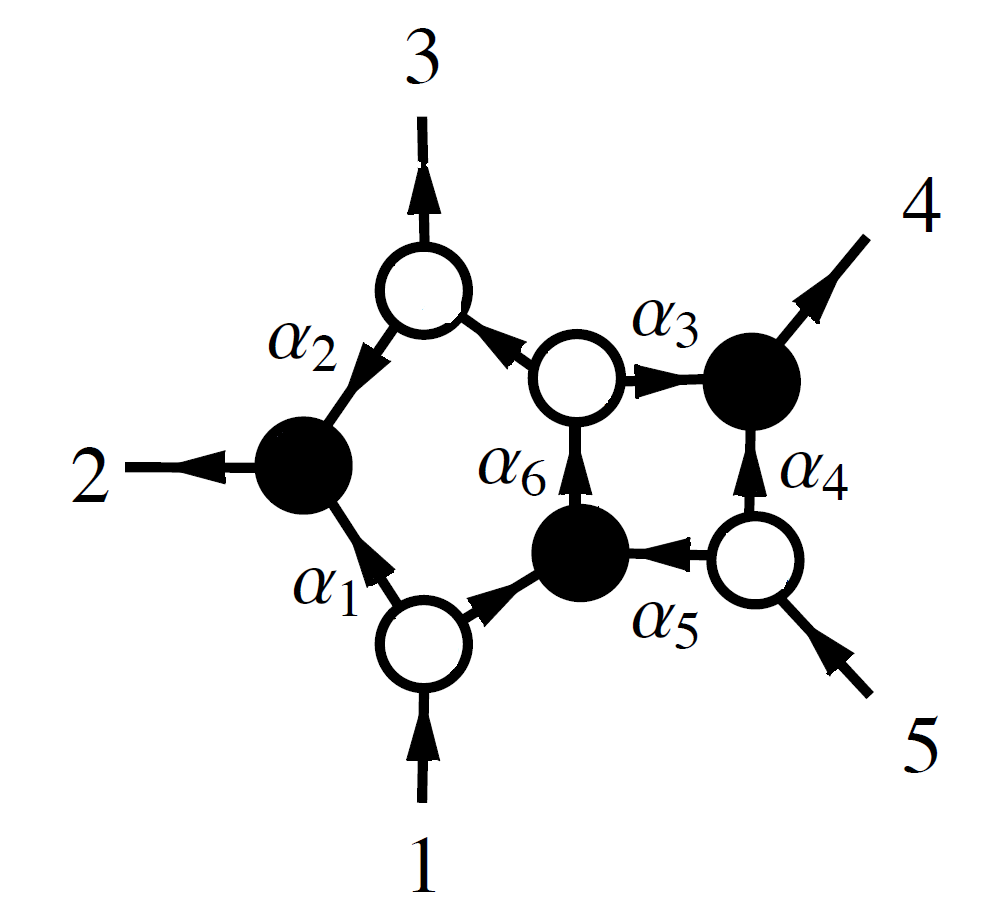
\includegraphics[width=0.25\linewidth]{5pt}
	\caption{Five point on-shell diagram}
	\label{fig:5pt}
\end{figure}
%\begin{figure}[H]\centering\hspace*{3cm}
%	\begin{tikzpicture}
%		\begin{scope}[very thick, every node/.style={sloped,allow upside down}]
%			\draw[black,fill=gray] (0,0) circle (2.4mm);
%			\draw (1.5,0) circle (2.4mm);
%			\draw[black,fill=gray] (1.5,1.5) circle (2.4mm);
%			\draw (0,1.5) circle (2.4mm);
%			\draw (-1.1,2.25) circle (2.4mm);
%			\draw (-1.1,-0.7) circle (2.4mm);
%			\draw (-2.5,0.75)[black,fill=gray]  circle (2.4mm);
%			\draw[thick,black] (1.25,0) -- node {\midarrow} (0.25,0);
%			\node[text width=0.5cm] at (0.75,-0.3) {$\alpha_3$};
%			\draw[thick,black] (1.25,1.5)  -- node {\midarrow}  (0.25,1.5);
%			\node[text width=0.5cm] at (0.75,1.8) {$\alpha_1$};
%			\draw[thick,black] (0,1.25) -- node {\midarrow} (0,0.25);
%			\node[text width=0.5cm] at (-0.3,0.75) {$\alpha_6$};
%			\draw[thick,black] (1.5,0.25) -- node {\midarrow} (1.5,1.25);
%			\node[text width=0.5cm] at (1.95,0.75) {$\alpha_2$};
%			\draw[thick,black] (1.5,0.25) -- node {\midarrow} (1.5,1.25);
%			\draw[thick,black] (-1.3,-0.6) -- node {\midarrow} (-2.35,0.56);
%			\node[text width=0.5cm] at (-2.1,-0.3) {$\alpha_1$};
%			\draw[thick,black] (-1.3,2.1) -- node {\midarrow} (-2.35,0.95);
%			\node[text width=0.5cm] at (-2.1,1.8) {$\alpha_2$};
%			%			
%			\draw[thick,black] (-0.18,-0.18) -- node {\midarrow} (-0.9,-0.6);
%			\draw[thick,black] (-3.55,0.75) -- node {\midarrow} (-2.75,0.74);
%			\draw[thick,black] (1.67,1.67) --  node {\midarrow} (2.2,2.2);
%			\draw[thick,black] (-0.9,2.1) -- node {\midarrow} (-0.19,1.67);
%			\draw[thick,black] (2.2,-0.7) -- node {\midarrow} (1.65,-0.17);
%			\draw[thick,black] (-1.11,-2.25) -- node {\midarrow} (-1.11,-0.95);
%			\draw[thick,black] (-1.11,3.75) -- node {\midarrow} (-1.11,2.5);
%			\draw (-0.5,0.75) circle (30.5mm);
%			%\node[text width=3cm] at (0.4,2.4) {1};
%			\node[text width=3cm] at (3.9,2.4) {4};
%			\node[text width=3cm] at (3.9,-0.9) {5};
%			%\node[text width=3cm] at (0.4,-0.9) {4};
%		\end{scope}
%	\end{tikzpicture}
%\end{figure}
\noindent
The $C$ matrix is
\begin{equation}
	\begin{aligned}
		C=\begin{pmatrix}
			1 & \alpha_1+\alpha_2\alpha_6 & \alpha_6 & \alpha_3\alpha_6 & 0\\
			0 & \alpha_5 \alpha_6 \alpha_2 & \alpha_5 \alpha_6 & \alpha_4+\alpha_3\alpha_5\alpha_6 & 1
		\end{pmatrix}
	\end{aligned}
\end{equation}
with the inverse being
\begin{equation}
	\begin{aligned}
		C^\perp =\begin{pmatrix}
			-(\alpha_1+\alpha_2\alpha_6) & 1 & 0 & 0 & -\alpha_5 \alpha_6 \alpha_2\\
			-\alpha_6 & 0 & 1 & 0 & -\alpha_5 \alpha_6 \\
			-\alpha_3 \alpha_6 & 0 & 0 & 1 & -(\alpha_4+\alpha_3\alpha_5\alpha_6)
		\end{pmatrix}
	\end{aligned}
\end{equation}
The amplitude is found through
\begin{equation}
	\begin{aligned}
		\dd \Omega =\frac{\dd \alpha_1}{\alpha_1}\frac{\dd \alpha_2}{\alpha_2}\frac{\dd \alpha_3}{\alpha_3}\frac{\dd \alpha_4}{\alpha_4}\frac{\dd \alpha_5}{\alpha_5}\frac{\dd \alpha_6}{\alpha_6}\delta(C\cdot \tilde \lambda) \delta(C^\perp\cdot \lambda)\delta(C\cdot \tilde \eta)
	\end{aligned}
\end{equation}
Using the delta-function $\delta(C^\perp\cdot \lambda)$ to solve for the $\alpha$'s we obtain, after contracting with $\lambda_1$, $\lambda_3$, and $\lambda_5$,
\begin{equation}
	\begin{aligned}
		\alpha_1=\frac{\expval{23}}{\expval{13}},~~~~
		\alpha_2=\frac{\expval{12}}{\expval{13}},~~~~
		\alpha_3=\frac{\expval{45}}{\expval{35}},~~~~
		\alpha_4=\frac{\expval{34}}{\expval{34}},~~~~
		\alpha_5=\frac{\expval{13}}{\expval{35}},~~~~
		\alpha_6=\frac{\expval{35}}{\expval{15}}
	\end{aligned}
\end{equation}
From which we get a Jacobian of $\frac{1}{\expval{15}^2\expval{13}}$. Plugging these $\alpha$'s back into $\delta (C\cdot\tilde \lambda)$, we get
\begin{equation}
	\begin{aligned}
0=&\tilde\lambda_1
+
\tilde\lambda_2 \frac{\expval{25}}{\expval{15}}
+
\tilde\lambda_3
\frac{\expval{35}}{\expval{15}}
+
\tilde\lambda_4
\frac{\expval{45}}{\expval{15}}\\
0=&\tilde\lambda_2 \frac{\expval{12}}{\expval{15}}
+
\tilde\lambda_3
\frac{\expval{13}}{\expval{15}}
+
\tilde\lambda_4 \frac{\expval{14}}{\expval{15}}
+
\tilde\lambda_5
\end{aligned}
\end{equation}
where we have used Schouten identities on the $\tilde\lambda_2$ term in the first equation and $\tilde \lambda_4$ term in the second equation. We find that
\begin{equation}
	\begin{aligned}
		\delta(C\cdot\lambda)=\expval{15}^2\delta (P)
	\end{aligned}
\end{equation}
Then we plug the $\alpha$'s into the Grassmann delta function. This will of course give a similar result with the exchange of $\tilde\lambda\to \tilde\eta$, although with the Jacobian factor now being $\frac{1}{\expval{15}^4}$. Finally we calculate
\begin{equation}
	\begin{aligned}
		\prod_i\frac{1}{\alpha_i}=\frac{\expval{13} \expval{15}^2 \expval{35}^2}{\expval{12}\expval{23}\expval{34}\expval{45}\expval{51}}
	\end{aligned}
\end{equation}
From which we are now easily able to get the form
\begin{equation}
	\begin{aligned}
		\dd \Omega =
		\frac{\delta^{8}\left(\mathcal{Q}\right)\delta^{4}\left(P\right)}{\expval{12}\expval{23}\expval{34}\expval{45}\expval{51}}
	\end{aligned}
\end{equation}
\subsection{Six-point NMHV}
For the NMHV ($k=3$) amplitude at six-points we get three different diagrams. In our case we will look at
\begin{figure}[H]
	\centering
	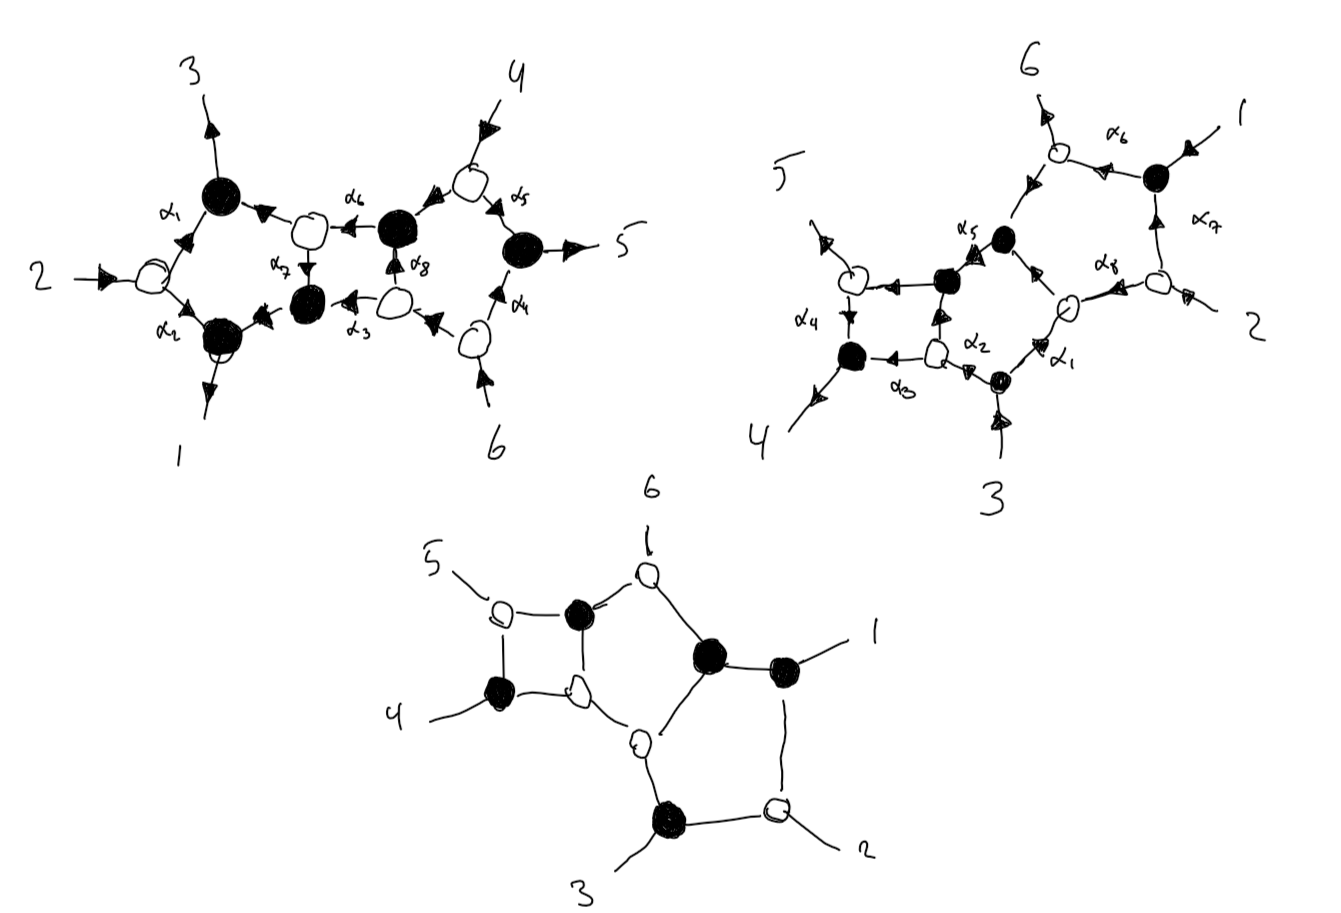
\includegraphics[width=0.9\linewidth]{nmhv}
	\caption[]{Diagrams contributing to the six point NMHV six point amplitude}
	\label{fig:44}
\end{figure}
\noindent
We first look at the 4+4 diagram, which has the following C-matrices
% TODO: \usepackage{graphicx} required
\begin{equation}
	\begin{aligned}
		C=\begin{pmatrix}
			\alpha_2 & 1 & \alpha_1 & 0 & 0 & 0\\
			\alpha_6 \alpha_7 & 0 &\alpha_6 & 1 & \alpha_5 & 0\\
			\alpha_3+\alpha_6\alpha_7\alpha_8 & 0 & \alpha_6\alpha_8  & 0 & \alpha_4 & 1
		\end{pmatrix},~~~~	C^\perp=\begin{pmatrix}
		1 & -\alpha_2 & 0 &-\alpha_6 \alpha_7 & 0 & -\alpha_3-\alpha_6\alpha_7\alpha_8\\
		0  & -\alpha_1 & 1 & -\alpha_6 & 0 & -\alpha_6\alpha_8\\
		0 & 0 & 0  & -\alpha_5 & 1 & -\alpha_4
	\end{pmatrix}
	\end{aligned}
\end{equation}
We then use the following combination of equation from the $C\cdot\tilde \lambda$ and $C_\perp\cdot \lambda$ delta functions
\begin{equation}
	\begin{aligned}
0=&-\langle 2 3 \rangle + \alpha_{4} \langle 2 4 \rangle,~~~~&&
0=-(\alpha_{5} \langle 2 4 \rangle) + \langle 3 4 \rangle
\\
0=&\left[ 6 1 \right] - \alpha_{2} \left[ 1 5 \right],~~~~&&
0=\left[ 6 5 \right] + \alpha_{1} \left[ 1 5 \right]
\\
0=&-\left[ 1 2 \right] - \alpha_{5} \left[ 1 3 \right] - \alpha_{6} \alpha_{7} \left[ 1 5 \right],~~~~&&
0=\alpha_{6} \left[ 1 5 \right] + \left[ 2 5 \right] + \alpha_{5} \left[ 3 5 \right]
\\
0=&-(\alpha_{4} \left[ 1 3 \right]) - \left[ 1 4 \right] - ( \alpha_{3} + \alpha_{6} \alpha_{7} \alpha_{8}) \left[ 1 5 \right],~~~~&&
0=\alpha_{6} \alpha_{8} \left[ 1 5 \right] + \alpha_{4} \left[ 3 5 \right] + \left[ 4 5 \right]
	\end{aligned}
\end{equation}
to obtain
\begin{align*}
	& \alpha_1 = -\frac{[65]}{[15]}\,, \quad \alpha_2 = \frac{[61]}{[15]}\,, \quad \alpha_3 = \frac{\sab{234}}{\aMs{4}{Q_{234}}{5}}\,, \quad \alpha_4 = \frac{\ab{23}}{\ab{24}}\,, \quad
	\alpha_5 = \frac{\ab{34}}{\ab{24}}\,, \\ 
	& \twhite{.}\hspace{1.4cm} 
	\alpha_6 = \frac{\aMs{4}{Q_{234}}{5}}{\ab{24}\sqb{15}}\,, \alpha_7 = -\frac{\aMs{4}{Q_{234}}{1}}{\aMs{4}{Q_{234}}{5}}\,,\quad
	\alpha_8 = - \frac{\aMs{2}{Q_{234}}{5}}{\aMs{4}{Q_{234}}{5}}\,.
\end{align*}
where $Q_{ijk}=p_i+p_j+p_k$
%%%%%%%%%%%%%%%%%%%%%%%%%%%%%%%%%%%%%%%%%%%%%%%%%%%%%%%%%%%%%%%%%%%%%%%%%%%%%%%%%%%%%%%%%%%%%%%%%%%%%%%%%%%%%%%%%%%%%%%%%%%%%%%%%%%%%%%%%%%%%%%%%%%%%%%%%%%%%%%%%%%%%%%%%%%%%%%%
For the other delta functions we get
\begin{equation}
	\begin{aligned}
	 0&=\tilde\eta_1-\frac{[65]}{[15]}\tilde\eta_2+\frac{[61]}{[15]}\tilde\eta_6\\
		0&= \frac{\langle4|Q_{234}|5]}{\expval{24}[15]}\tilde\eta_1+\tilde\eta_2+\frac{\expval{34}}{\expval{24}}\tilde\eta_4-\frac{\langle3|Q_{234}|1]}{\expval{24}[15]}\tilde\eta_6
		\\
		0&= -\frac{\langle2|Q_{234}|5]}{\expval{24}[15]}\tilde\eta_2+\frac{\expval{23}}{\expval{24}}\tilde\eta_4+\tilde\eta_5+\frac{s_{234}\expval{24}[15]+\langle2|Q_{234}|5]\langle4|Q_{234}|1] }{\langle4|Q_{234}|5]}
\tilde\eta_5
	\end{aligned}
\end{equation}
The Jacobian from the delta functions is
\begin{equation}
	\begin{aligned}
		J=\frac{1}{[15]^3\expval{24}^3\aMs{4}{Q_{234}}{5}^2}
	\end{aligned}
\end{equation}
and we get the form
\begin{equation}
	\begin{aligned}
		\dd \Omega_1=\frac{\delta(\sum P)\delta(\tilde\eta_5[16]+\tilde\eta_6[15]+\tilde\eta_1[56])}{s_{234}\expval{23}\expval{34}[61][56]\aMs{2}{Q_{234}}{5}\aMs{4}{Q_{234}}{1}}
	\end{aligned}
\end{equation}
Looking at the 5+3 diagram we get the following C-matrix
\begin{equation}
	\begin{aligned}
		C&=\left(
		\begin{array}{cccccc}
		\alpha_7 &1& \alpha_8(\alpha_1+\alpha_2\alpha_5)&\alpha_3\alpha_5\alpha_8& 0& 0 \\
		0 &0&\alpha_2 & \alpha_3+\alpha_4 & 1 & 0 \\
		\alpha_6 & 0& \alpha_2\alpha_5& \alpha_3\alpha_5 &0 & 1 \\
		\end{array}
		\right)\\
		C_\perp&=
		\left(
		\begin{array}{cccccc}
		1 & -\alpha_7 & 0 & 0 & 0& -\alpha_6  \\
		0 & -\alpha_8(\alpha_1+\alpha_2\alpha_5) & 1 &0 & -\alpha_2 & -\alpha_2\alpha_5 \\
		0 & -\alpha_3\alpha_5\alpha_8 & 0 &1 &-\alpha_3-\alpha_4 &-\alpha_3\alpha_5 
		\end{array}
		\right)
	\end{aligned}
\end{equation}
From the delta functions $\delta(C\cdot \tilde \lambda)$ and $\delta(C_\perp \cdot \lambda)$, we use the following equations
\begin{equation}
	\begin{aligned}
		0=&\langle 2 6 \rangle - (\alpha_{3} + \alpha_{4}) \langle 3 6 \rangle - \alpha_{3} \alpha_{5} \langle 4 6 \rangle,~~~~
		&&0=-\langle 4 5 \rangle + \alpha_{7} \langle 4 6 \rangle,\\
	0=&	-\alpha_{6} \langle 4 6 \rangle + \langle 5 6 \rangle
	,~~~~
	&&0=	-(\alpha_{3} + \alpha_{4}) \left[ 1 2 \right] - \left[ 1 3 \right],
		\\
	0=&	\alpha_{2} \left[ 1 2 \right] - \left[ 2 3 \right],~~~~
	&&0=	\alpha_{2} \alpha_{5} \left[ 1 2 \right] - \left[ 2 4 \right] - \alpha_{6} \left[ 2 5 \right],
		\\
	0=&	-\alpha_{3} \alpha_{5} \alpha_{8} \left[ 1 2 \right] - \alpha_{7} \left[ 1 5 \right] - \left[ 1 6 \right],~~~~
	&&0=	(\alpha_{1} + \alpha_{2} \alpha_{5}) \alpha_{8} \left[ 1 2 \right] - \alpha_{7} \left[ 2 5 \right] - \left[ 2 6 \right],
	\end{aligned}
\end{equation}
to obtain solutions for the edge-variables
\begin{equation}
	\begin{aligned}
			& \alpha_1 = \frac{\sab{612}}{\aMs{6}{Q_{612}}{3}}\,, \quad \alpha_2 = \frac{[45]}{[34]}\,, \quad \alpha_3 = \frac{[45]\aMs{2}{Q_{612}}{3}}{[34]\aMs{2}{Q_{612}}{4}}\,, \quad \alpha_4 = \frac{\aMs{2}{Q_{612}}{5}}{\aMs{2}{Q_{612}}{4}}\,,\\ 
		&\alpha_5 = \frac{\aMs{2}{Q_{612}}{4}}{\ab{62}[45]}\,, 
		 \quad
		\alpha_6 = \frac{\ab{12}}{\ab{62}}\,,\quad \alpha_7 = \frac{\ab{61}}{\ab{62}}\,,\quad
		\alpha_8 =  \frac{\aMs{6}{Q_{612}}{3}}{\aMs{2}{Q_{612}}{3}}\,.
	\end{aligned}
\end{equation}
Here the Jacobian from the delta functions is
\begin{equation}
	\begin{aligned}
		J=\frac{1}{[34]^3\expval{62}^3\aMs{2}{Q_{612}}{4}\aMs{6}{Q_{612}}{3}}
	\end{aligned}
\end{equation}
and we get the form
\begin{equation}
	\begin{aligned}
		\dd \Omega_2=\frac{\delta(\sum P)\delta(\tilde\eta_3[45]+\tilde\eta_4[35]+\tilde\eta_5[34])}{s_{612}\expval{12}\expval{16}[34][35]\aMs{6}{Q_{612}}{3}\aMs{2}{Q_{612}}{5}}
	\end{aligned}
\end{equation}
The final diagram can be found by permuting by $2$ and exchanging square and angle brackets:
\begin{equation}
	\begin{aligned}
		\dd \Omega_3=\frac{\delta(\sum P)\delta(\tilde\eta_1[23]+\tilde\eta_2[13]+\tilde\eta_3[12])}{s_{456}\expval{45}\expval{56}[23][12]\aMs{4}{Q_{456}}{1}\aMs{6}{Q_{456}}{3}}
	\end{aligned}
\end{equation}
In total we have
\begin{equation}
	\begin{aligned}
		&\dd \Omega_1 +\dd \Omega_2+\dd \Omega_3\\
		=&\frac{\delta(\sum P)\delta(\tilde\eta_5[16]+\tilde\eta_6[15]+\tilde\eta_1[56])}{s_{234}\expval{23}\expval{34}[61][56]\aMs{2}{Q_{234}}{5}\aMs{4}{Q_{234}}{1}}
		+\frac{\delta(\sum P)\delta(\tilde\eta_3[45]+\tilde\eta_4[35]+\tilde\eta_5[34])}{s_{612}\expval{12}\expval{16}[34][35]\aMs{6}{Q_{612}}{3}\aMs{2}{Q_{612}}{5}}
		\\&+\frac{\delta(\sum P)\delta(\tilde\eta_1[23]+\tilde\eta_2[13]+\tilde\eta_3[12])}{s_{456}\expval{45}\expval{56}[23][12]\aMs{4}{Q_{456}}{1}\aMs{6}{Q_{456}}{3}}
	\end{aligned}
\end{equation}
Then using the fact that
\begin{eqnarray}
	&&  \sA^{(0),\text{MHV}} R_{j,j+3,j+5} =\nonumber\\
	&&\hskip 5mm \frac{%
		\delt8\bigl(\sum \lambda_i \eta^A_i\bigr)
	}
	{\spa{j}.{(j\tp 1)} \spa{(j\tp 1)}.{(j\tp 2)}\spb{(j\tp 3)}.{(j\tp 4)}
		\spb{(j\tp 4)}.{(j\tp 5)}}\\
	&&\hskip 5mm \times\frac{\delt4\bigl(\eta^A_{j+3} \spb{(j\tp4)}.{(j\tp5)} 
		+ \eta^A_{j+4} \spb{(j\tp5)}.{(j\tp3)} 
		+ \eta^A_{j+5} \spb{(j\tp3)}.{(j\tp4)}\bigr)}
	{\sandmx{j}.{K_{j+1,j+2}}.{(j\tp 3)}
		\sandmx{(j\tp 2)}.{K_{j+3,j+4}}.{(j\tp 5)}
		s_{j,j+1,j+2}}\,.\nonumber
\end{eqnarray} 
We find that the full NMHV amplitude can be written as
\begin{equation}
	\begin{aligned}
		A_6^{\text{NMHV}}=A_6^{\text{MHV}}\left(R_{251}+R_{413}+R_{635}\right)
	\end{aligned}
\end{equation}
Having now showed the general procedure to calculate forms from the on-shell diagrams, we will show how to extend this approach to amplitudes with $\mathcal{N}\neq 4$ super-symmetries. 
\newpage
\section{Calculating $\mathcal{N}<4$ amplitudes\label{sec:YM}} 
\subsection{The measure}
Since going to $\mathcal{N}<4$ means that the graphs have to be oriented, one has to consider all internal orientations for specific external helicity configurations. Further, for diagrams containing closed internal loops, one has to add an extra factor, $\mathcal{J}$ , in
the measure,
\begin{equation}
	\begin{aligned}
		\dd \Omega= \dlog{\alpha_1} \dlog{\alpha_2}\cdots  \dlog{\alpha_m} \mathcal{J}^{\mathcal{N}-4} \delta(C\cdot Z),
	\end{aligned}
\end{equation}
where this Jacobian is given by
\begin{equation}
	\begin{aligned}
		\mathcal{J}=1+\sum_if_i+\sum_{\substack{\text{disjoint}\\ \text{pairs } i,j}}f_i f_j+\sum_{\substack{\text{disjoint}\\ \text{pairs } i,j,k}}f_i f_j f_k+\cdots
	\end{aligned}
\end{equation}
with $f_i$ denoting the face of a closed cycle, and the sums are over disjoint collections of these closed cycles. One also has to note that each face is defined as \textit{clockwise-oriented product of edge-variables}, meaning that a counterclockwise cycle would produce $\frac{1}{f}$.
In the following sections we will specifically consider $\mathcal N=0$ for which one also has to take $\delta(C\cdot Z)=\delta(C^\perp\cdot \lambda)\delta(C\cdot \tilde\lambda)$.
\subsection{Four-point $\mathcal{N}=0$ with internal loop}
The simplest example is at four points where we have two diagrams after fixing the external helicities
\begin{figure}[H]
	\centering
	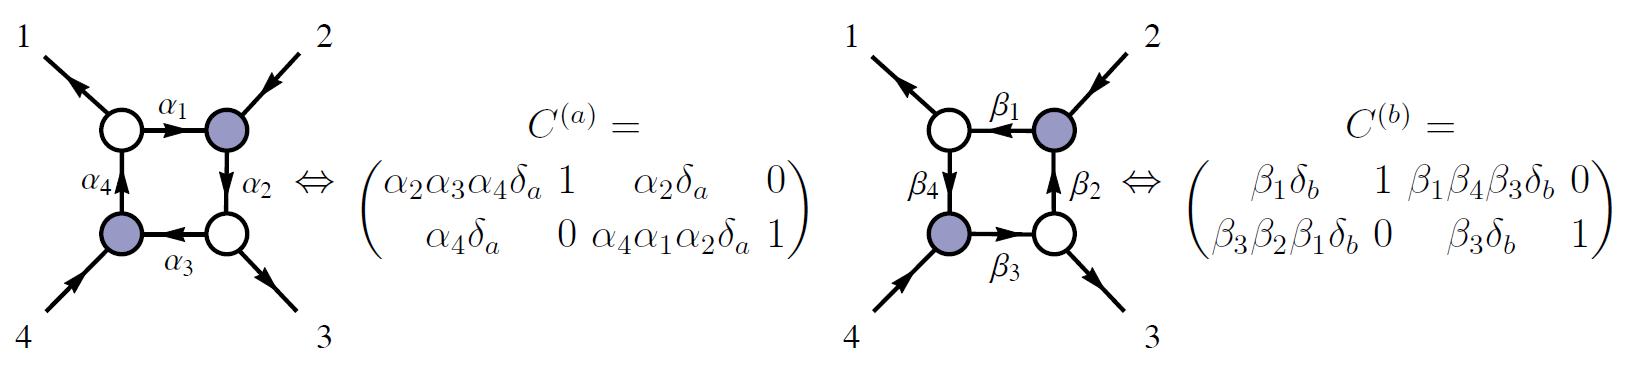
\includegraphics[width=0.7\linewidth]{YM4pt}
	\caption{All diagrams contributing to the specified helicity configuration at four points}
	\label{fig:jexample}
\end{figure}
where the $\delta's$ are defined by
\begin{equation}
	\begin{aligned}
		\delta_a=\frac{1}{1-\prod_{i=1}^{4}\alpha_i},~~~~~~\delta_b=\frac{1}{1-\prod_{i=1}^{4}\beta_i}
	\end{aligned}
\end{equation}
Solving the $C_\perp$ delta-function, we get the following equations after contracting with $\lambda_2$ and $\lambda_4$
\begin{equation}
	\begin{aligned} \label{eq:1}
		           0&=   
		\langle 1 2 \rangle + \frac{ \alpha_{4} \langle 2 4\rangle
		}{1 - \alpha_{1} \alpha_{2} \alpha_{3} \alpha_{4}},~~~~&&
 0=   
\langle 1 4\rangle - \frac{\alpha_{2} \alpha_{3} \alpha_{4} \langle 2 4\rangle
}{1 - \alpha_{1} \alpha_{2} \alpha_{3} \alpha_{4}},
\\
 0&=   
-\langle 23\rangle + \frac{\alpha_{1} \alpha_{2} \alpha_{4} \langle 2 4\rangle
}{1 - \alpha_{1} \alpha_{2} \alpha_{3} \alpha_{4}}
,~~~~&&
	 0=   
	\langle 3 4\rangle - \frac{\alpha_{2}  \langle 2 4\rangle
	}{1 - \alpha_{1} \alpha_{2} \alpha_{3} \alpha_{4}}
	\end{aligned}
\end{equation}
from which we obtain
\begin{equation}
	\begin{aligned} \label{eq:1}
	\alpha_1&=-\frac{\langle 23 \rangle}{\langle 13\rangle},~~~~~~~~~~\alpha_2=\frac{\langle 13 \rangle}{\langle 12\rangle},\\
	\alpha_3&=-\frac{\langle 14 \rangle}{\langle 13\rangle},~~~~~~~~~~	\alpha_4=-\frac{\langle 13 \rangle}{\langle 34\rangle},
	\end{aligned}
\end{equation}
along with a Jacobian factor from rewriting the delta functions of $\frac{\ab{24}^2}{\ab{12}^2\ab{34}^2}$.
We further find an expression for $\delta_a$
\begin{equation}
	\begin{aligned}
\delta_a=\frac{\langle 1 2 \rangle \langle 34 \rangle}{ \langle 13 \rangle\langle 24 \rangle}
	\end{aligned}
\end{equation}
Taking these solutions and inserting into the other delta functions, and multiplying by $\tilde\lambda_1$ and $\tilde\lambda_3$ we get
\begin{equation}
	\begin{aligned}
	0&=	\sqb{12}+\frac{\ab{34}\sqb{13}}{\ab{24}}
,	~~~~~~~~
	0=	\sqb{23}+\frac{\ab{14}\sqb{13}}{\ab{24}}
	\\
	0&=	\sqb{14}+\frac{\ab{23}\sqb{13}}{\ab{24}}
,	~~~~~~~~
	0=	\sqb{34}+\frac{\ab{12}\sqb{13}}{\ab{24}}
	\end{aligned}
\end{equation}
which we can combine into $\delta^4(P)\ab{24}^2$. Finally the Jacobian is
\begin{equation}
	\begin{aligned}
		\mathcal{J}_a=1-\alpha_{1}\alpha_{2}\alpha_{3}\alpha_{4}=\delta_a^{-1}=
		\frac{ \langle 13 \rangle\langle 24 \rangle}{\langle 1 2 \rangle \langle 34 \rangle}
	\end{aligned}
\end{equation}
The procedure is the same for the other diagram and here we just summarize the results
\begin{equation}
	\begin{aligned}
		\beta_1&=\frac{\langle 13 \rangle}{\langle 23\rangle},~~~~~~~~~~\beta_2=\frac{\langle 21 \rangle}{\langle 13\rangle},\\
		\beta_3&=\frac{\langle 13 \rangle}{\langle 14\rangle},~~~~~~~~~~	\beta_4=\frac{\langle 34 \rangle}{\langle 13\rangle},
	\end{aligned}
\end{equation}
\begin{equation}
	\begin{aligned}
		\mathcal{J}_b=1-\beta_{1}\beta_{2}\beta_{3}\beta_{4}=\delta_b^{-1}=
		\frac{ \langle 13 \rangle\langle 24 \rangle}{\langle 1 4 \rangle \langle 23 \rangle}
	\end{aligned}
\end{equation}
Combining all these factors with $\prod_i \alpha_i=\frac{\ab{41}\ab{23}}{\ab{12}\ab{34}}$ and $\prod_i \beta_i=\frac{\ab{12}\ab{34}}{\ab{23}\ab{41}}$, as well as using taking the Jacobians to the $-4$'th power, we can combine them in the form
\begin{equation}
	\begin{aligned}
		\dd \Omega &=\frac{\ab{24}^4}{\ab{12}\ab{23}\ab{34}\ab{41}}\left( \left[\frac{ \langle 13 \rangle\langle 24 \rangle}{\langle 1 2 \rangle \langle 34 \rangle}\right]^{-4}+\left[	\frac{ \langle 13 \rangle\langle 24 \rangle}{\langle 1 4 \rangle \langle 23 \rangle}\right]^{-4}\right)\delta(P)\\
	\end{aligned}
\end{equation}
\subsection{Five-point $\mathcal{N}=0$, no internal cycle}
For five and six points we will look at two different types of diagrams. First we analyze one without an internal cycle, i.e. has $\mathcal{J}=1$. As will be evident, this produces  the standard Yang-Mills amplitude. We then follow this by evaluating diagrams with internal cycles, which can be used to get forms for $\mathcal{N}\neq4$.
We will once again look at the following diagram
\begin{figure}[H]
	\centering
	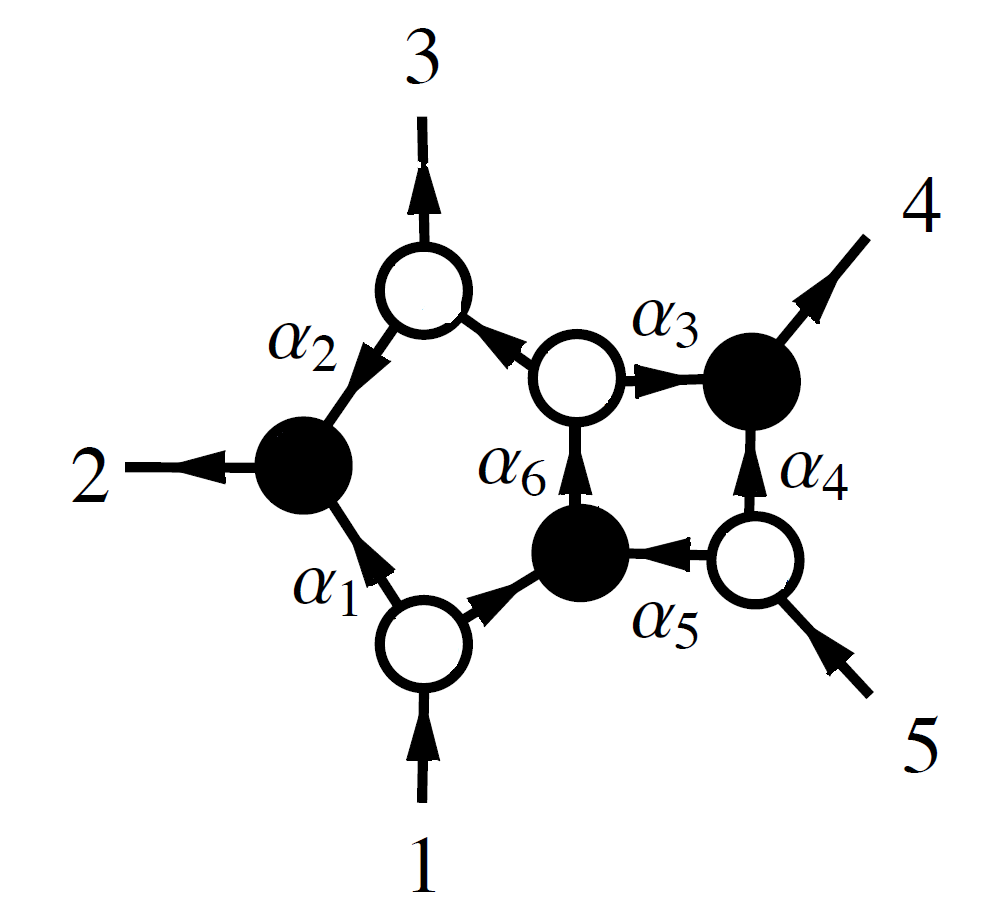
\includegraphics[width=0.3\linewidth]{5pt}
	\caption{Five point on-shell diagram}
	\label{fig:5pt}
\end{figure}
We already solved this in section \ref{sec:examples}, here we obtained the following edge-variables after contracting with $\lambda_1$, $\lambda_3$, and $\lambda_5$
\begin{equation}
	\begin{aligned}
		\alpha_1=\frac{\expval{23}}{\expval{13}},~~~~
		\alpha_2=\frac{\expval{12}}{\expval{13}},~~~~
		\alpha_3=\frac{\expval{45}}{\expval{35}},~~~~
		\alpha_4=\frac{\expval{34}}{\expval{34}},~~~~
		\alpha_5=\frac{\expval{13}}{\expval{35}},~~~~
		\alpha_6=\frac{\expval{35}}{\expval{15}}
	\end{aligned}
\end{equation}
and a Jacobian from solving the delta functions of $\frac{\ab{15}^2}{\expval{35}^2\expval{13}}$. For this diagram we have two negative helicity particles $1$ and $5$ which is seen from the incoming arrows at those points. The orientation of these external legs do not yield an internal orientation with a closed cycle, and so this is the only diagram we have to take into account and there is no extra Jacobian factor. Using $\prod_{i}\alpha_i=\frac{\ab{12}\ab{23}\ab{34}\ab{45}}{\ab{13}\ab{15}\ab{35}^2}$ The form then yields the amplitude
\begin{equation}
	\begin{aligned}
		\dd \Omega_5(1^-,2^+,3^+,4^+,5^-)&=\frac{\ab{15}^2}{\expval{35}^2\expval{13}}\frac{\delta(P)}{\prod_i \alpha_i}\\
		&=\frac{\ab{15}^4}{\ab{12}\ab{23}\ab{34}\ab{45}\ab{51}}\delta(P)
	\end{aligned}
\end{equation}
\subsection{Five point with internal cycles}
We will now consider a diagram containing internal cycles. For the fixed helicity configuration of $(1^+,2^-,3^+,4^+,5^-)$ the diagrams below contribute
\begin{figure}[H]
	\centering
	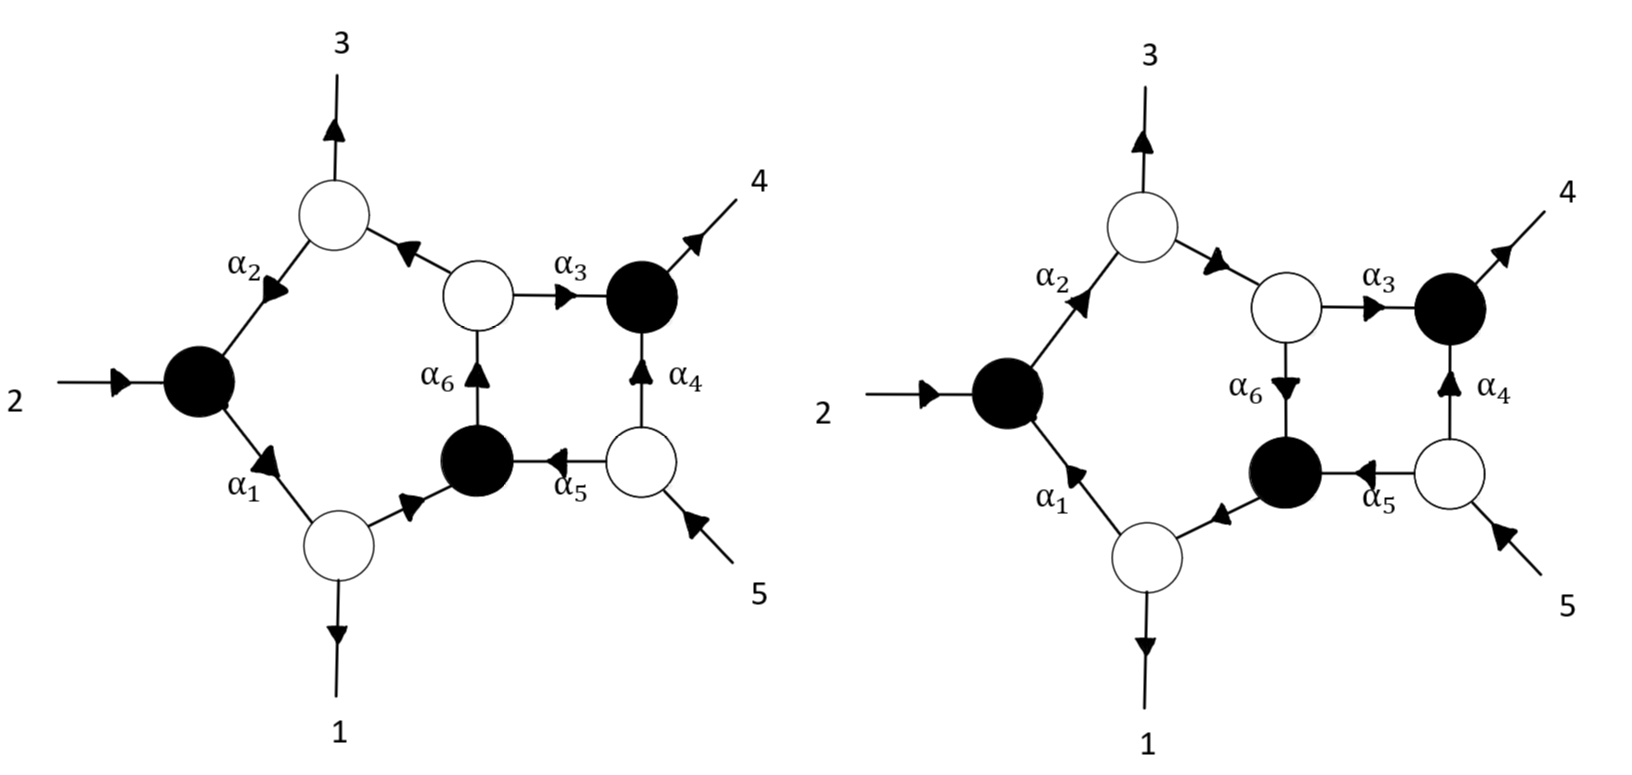
\includegraphics[width=0.7\linewidth]{5pt3}
	\caption{All diagrams for the specified five point helicity configuration}
	\label{fig:5pt}
\end{figure}
\noindent
Denoting the left diagram by "$a$" and the right one by "$b$", the $C$-matrices are
\begin{equation}
	\begin{aligned}
		C_a&=\left(
		\begin{array}{ccccc}
			\alpha _1 \delta_a & 1 & \alpha _1 \alpha _6 \delta_a & \alpha _1 \alpha _3 \alpha _6 \delta_a & 0 \\
	\alpha _1 \alpha _2 \alpha _5 \alpha _6 \delta_a & 0 & \alpha _5 \alpha _6 \delta_a & \alpha _3 \alpha _5 \alpha _6 \delta_a+\alpha _4 & 1 \\
		\end{array}
		\right)
		,~~~~
		C_a^\perp = \left(
		\begin{array}{ccccc}
			1 & -\alpha _1 \delta_a & 0 & 0 & -\alpha _1 \alpha _2 \alpha _5 \alpha _6 \delta_a \\
		0 & -\alpha _1 \alpha _6 \delta_a & 1 & 0 & -\alpha _5 \alpha _6 \delta_a \\
		0 & -\alpha _1 \alpha _3 \alpha _6 \delta_a & 0 & 1 & -\alpha _3 \alpha _5 \alpha _6 \delta_a-\alpha _4 \\
		\end{array}
		\right)\\
		C_b&=\left(
		\begin{array}{ccccc}
			\beta _2 \beta _6 \delta_b & 1 & \beta _2 \delta_b & \beta _2 \beta _3 \delta_b & 0 \\
			\beta _5 \delta_b & 0 & \beta _1 \beta _2 \beta _5 \delta_b & \beta _1 \beta _2 \beta _3 \beta _5 \delta_b+\beta _4 & 1 \\
		\end{array}
		\right),~~~~~~~C_b^\perp =
		\left(
		\begin{array}{ccccc}
			1 & -\beta _2 \beta _6 \delta_b & 0 & 0 & -\beta _5 \delta_b \\
			0 & -\beta _2 \delta_b & 1 & 0 & -\beta _1 \beta _2 \beta _5 \delta_b \\
			0 & -\beta _2 \beta _3 \delta_b & 0 & 1 & -\beta _1 \beta _2 \beta _3 \beta _5 \delta_b -\beta _4 \\
		\end{array}
		\right)
	\end{aligned}
\end{equation}
Solving the delta-function constraints we are led to the following solutions for the edge variables
\begin{equation}
	\begin{aligned}
		&\alpha_1=\frac{\expval{13}}{\expval{23}},~~~~
		\alpha_2=-\frac{\expval{12}}{\expval{13}},~~~~
		\alpha_3=\frac{\expval{45}}{\expval{35}},~~~~
		\alpha_4=\frac{\expval{34}}{\expval{35}},~~~~
		\alpha_5=\frac{\expval{13}}{\expval{35}},~~~~
		\alpha_6=\frac{\expval{35}}{\expval{15}}\\
	&\beta_1=-\frac{\expval{23}}{\expval{13}},~~~~
	\beta_2=-\frac{\expval{13}}{\expval{12}},~~~~
	\beta_3=\frac{\expval{45}}{\expval{35}},~~~~
	\beta_4=\frac{\expval{34}}{\expval{35}},~~~~
	\beta_5=-\frac{\expval{13}}{\expval{35}},~~~~
	\beta_6=\frac{\expval{15}}{\expval{35}}
	\end{aligned}
\end{equation}
along with a Jacobian from solving the delta functions of $\frac{\ab{13}\ab{25}^4}{\ab{15}^2\ab{23}^2\ab{35}^2}$ and $\frac{\ab{13}\ab{25}^4}{\ab{12}^2\ab{35}^2}$ respectively. The Jacobians from the internal loops are
\begin{equation}
	\begin{aligned}
		\J_a=\delta_a^{-1}=\frac{\ab{13}\ab{25}}{\ab{15}\ab{23}},~~~~~~\J_b=\delta_b^{-1}=\frac{\ab{13}\ab{25}}{\ab{12}\ab{35}}
	\end{aligned}
\end{equation}
One can note that these can be rewritten using Schouten,
\begin{equation}
	\begin{aligned}
		\J_a=1+\frac{\ab{12}\ab{35}}{\ab{15}\ab{23}}\equiv1+f^{-1},~~~~\J_a=1+\frac{\ab{15}\ab{23}}{\ab{12}\ab{35}}\equiv1+f
	\end{aligned}
\end{equation}
and since, as we will se shortly, the forms produced by the individual diagrams only differ by this Jacobian, one does not have to go through the calculation of both diagrams, but can instead infer, the Jacobian by rewriting it in this form. Similarly we will also find that changing the direction of an arrow, just flips the expression for the edge $\alpha_k\to\frac{1}{\alpha_k}$, from which the Jacobian of the reverse cycle diagram can be found.

Using this, the $\mathcal{N}=0$ form for the cut is found by adding the diagrams
\begin{equation}
	\begin{aligned}
		\dd\Omega
		&=\left(\frac{\ab{13}\ab{25}^4}{\ab{15}^2\ab{23}^2\ab{35}^2}J_a^{-4}\prod_{i=1}^{5}\frac{1}{\alpha_i}+\frac{\ab{13}\ab{25}^4}{\ab{12}^2\ab{35}^2}J_b^{-4}\prod_{i=1}^{5}\frac{1}{\beta_i}\right)\delta(P)\\
		&=\frac{\ab{25}^4}{\ab{12}\ab{23}\ab{34}\ab{45}\ab{51}}\delta(P)\left(J_a^{-4}+J_b^{-4}\right)\\
		&=\frac{\ab{15}^4\ab{23}^4+\ab{12}^4\ab{35}^4}{\ab{13}^4\ab{12}\ab{23}\ab{34}\ab{45}\ab{51}}\delta(P)
	\end{aligned}
\end{equation}
As described, the only difference between the two diagrams is the Jacobian. To complete the picture we will consider one further example, by changing the external helicity configuration to $(1^-,2^+,3^+,4^-,5^+)$. Here the diagrams below contribute
\begin{figure}[H]
	\centering
	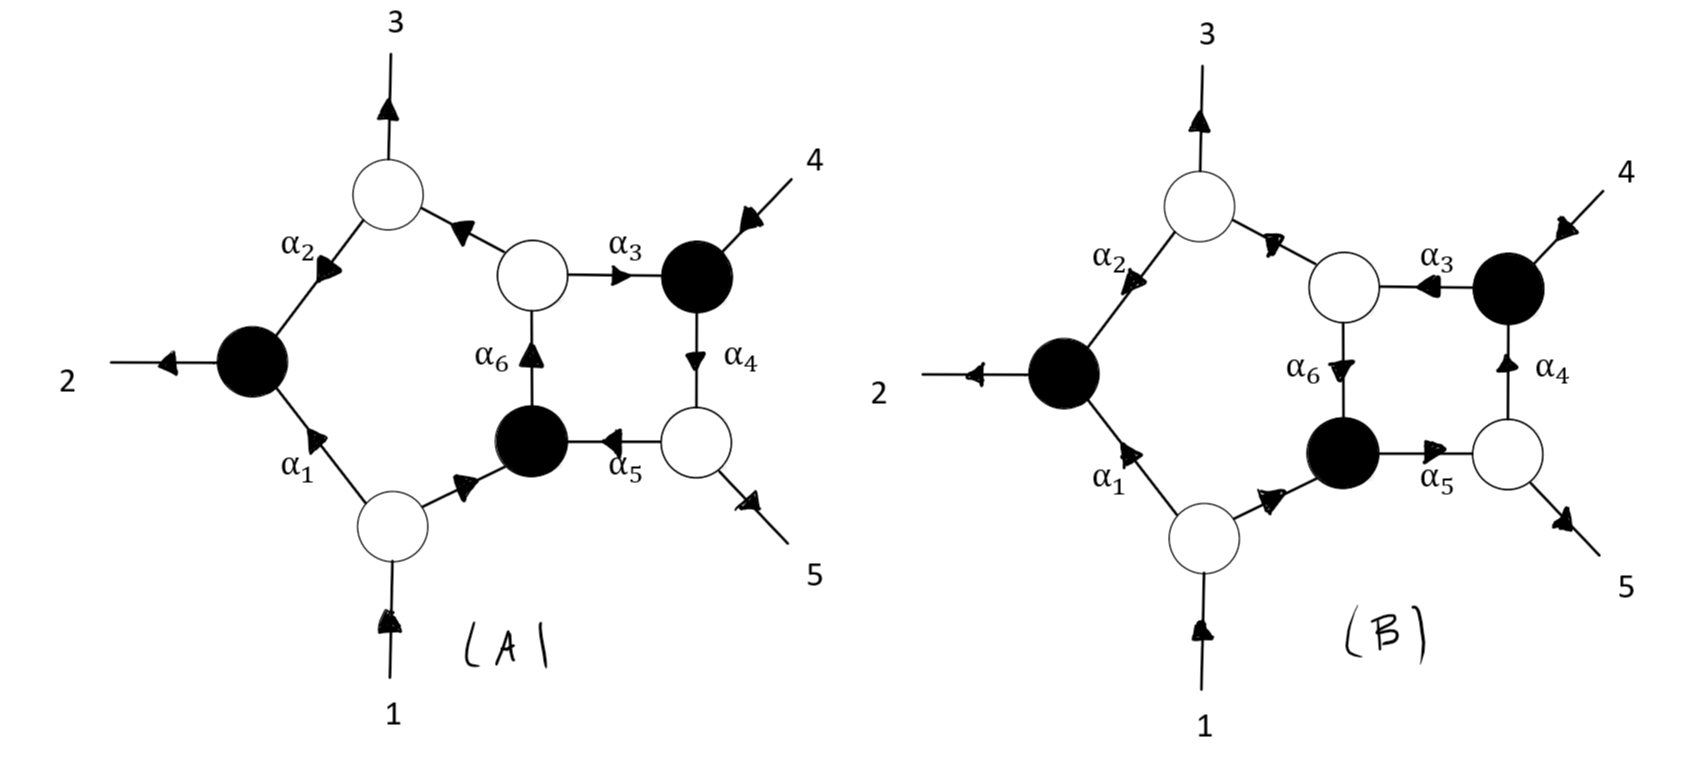
\includegraphics[width=0.7\linewidth]{5pt4}
	\caption{All diagrams for the specified five point helicity configuration}
	\label{fig:5pt}
\end{figure}
\noindent We will just consider the "$A$" diagram and then apply the above method to get the Jacobian from the "$B$" orientation.
We obtain
\begin{equation}
	\begin{aligned}
		C_A&=\left(
		\begin{array}{ccccc}
			1 & \alpha _2 \alpha _6 \delta_a +\alpha _1 & \alpha _6 \delta_a  & 0 & \alpha _3 \alpha _4 \alpha _6 \delta_a  \\
			0 & \alpha _2 \alpha _4 \alpha _5 \alpha _6 \delta_a  & \alpha _4 \alpha _5 \alpha _6 \delta_a  & 1 & \alpha _4 \delta_a  \\
		\end{array}
		\right)\\
		C_A^\perp &=\left(
		\begin{array}{ccccc}
			-\alpha _2 \alpha _6 \delta -\alpha _1 & 1 & 0 & -\alpha _2 \alpha _4 \alpha _5 \alpha _6\delta & 0 \\
			-\alpha _6 \delta  & 0 & 1 & -\alpha _4 \alpha _5 \alpha _6 \delta & 0 \\
			-\alpha _3 \alpha _4 \alpha _6 \delta  & 0 & 0 & -\alpha _4 \delta & 1 \\
		\end{array}
		\right)
	\end{aligned}
\end{equation}
\begin{equation}
	\begin{aligned}
		&\alpha_1=\frac{\expval{23}}{\expval{13}},~~~~
		\alpha_2=\frac{\expval{12}}{\expval{13}},~~~~
		\alpha_3=-\frac{\expval{45}}{\expval{35}},~~~~
		\alpha_4=\frac{\expval{35}}{\expval{34}},~~~~
		\alpha_5=\frac{\expval{13}}{\expval{35}},~~~~
		\alpha_6=\frac{\expval{35}}{\expval{15}}\\
		\end{aligned}
\end{equation}
with 
\begin{equation}
	\begin{aligned}
		J_a=\frac{\ab{14}\ab{35}}{\ab{15}\ab{34}},~~~~~~J_b=\frac{\ab{14}\ab{35}}{\ab{13}\ab{45}}
	\end{aligned}
\end{equation}
and the $\mathcal{N}=0$ form for the cut is found to be
\begin{equation}
	\begin{aligned}
		\dd \Omega
		=\frac{\ab{14}^4}{\ab{12}\ab{23}\ab{34}\ab{45}\ab{51}}\delta(P)\left(\left[\frac{\ab{14}\ab{35}}{\ab{15}\ab{34}}\right]^{-4}+\left[\frac{\ab{14}\ab{35}}{\ab{13}\ab{45}}\right]^{-4}\right)
	\end{aligned}
\end{equation}
\subsection{Six-point $\mathcal{N}=0$}
To illustrate what the form of the bare\footnote{By bare we mean the form without the internal cycle Jacobian} diagram should look like we start by treating a diagram without an internal cycle.  We take the same diagram as we did in section \ref{sec:examples}.
\begin{figure}[H]
	\centering
	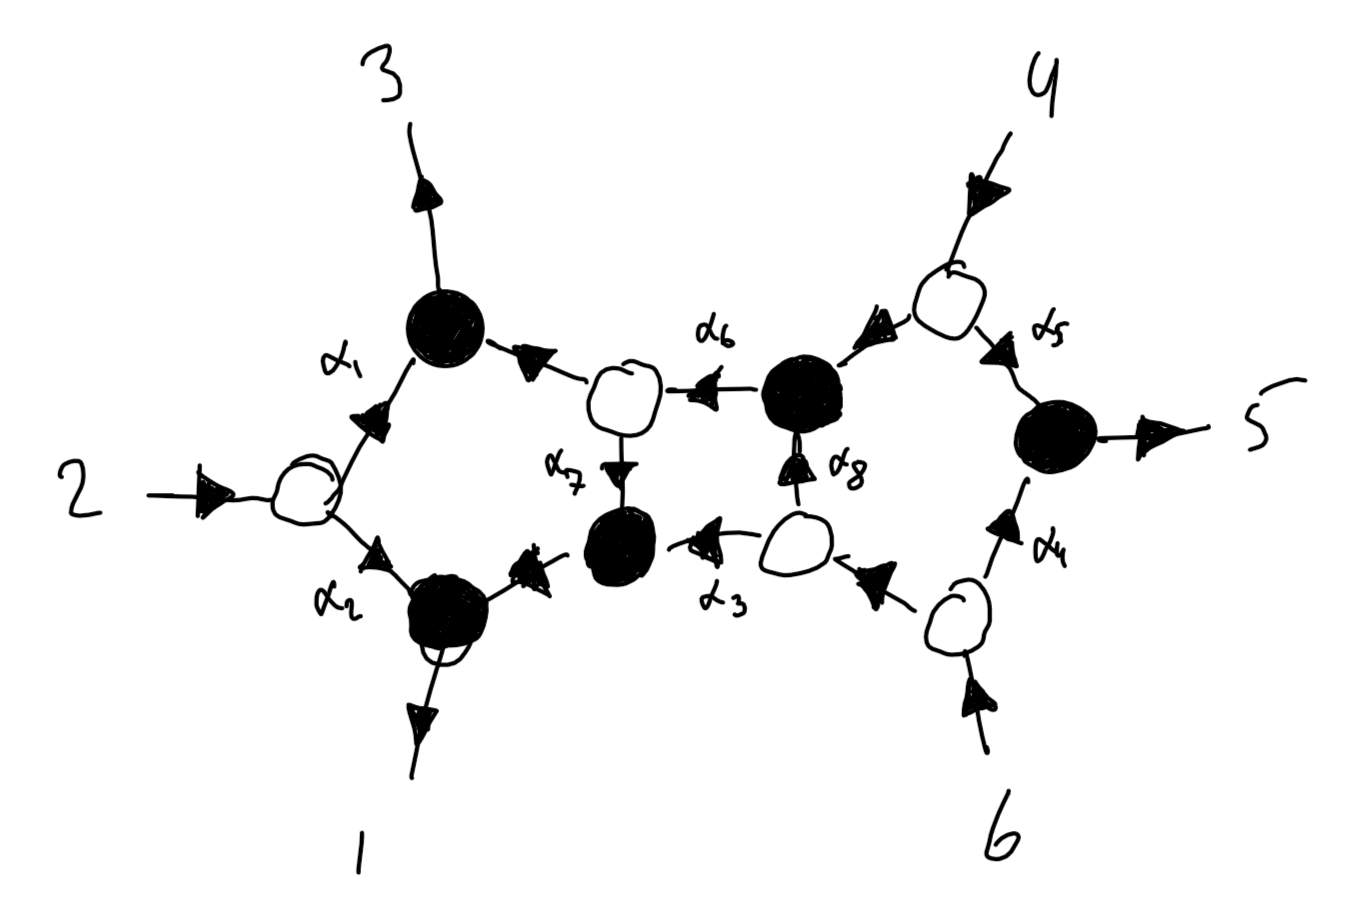
\includegraphics[width=0.4\linewidth]{6ptYM}
	\caption{4+4 NMHV six point diagram}
	\label{fig:5pt}
\end{figure}
\noindent where we obtained
\begin{align*}
	& \alpha_1 = -\frac{[65]}{[15]}\,, \quad \alpha_2 = \frac{[61]}{[15]}\,, \quad \alpha_3 = \frac{\sab{234}}{\aMs{4}{Q_{234}}{5}}\,, \quad \alpha_4 = \frac{\ab{23}}{\ab{24}}\,, \quad
	\alpha_5 = \frac{\ab{34}}{\ab{24}}\,, \\ 
	& \twhite{.}\hspace{1.4cm} 
	\alpha_6 = \frac{\aMs{4}{Q_{234}}{5}}{\ab{24}\sqb{15}}\,, \alpha_7 = -\frac{\aMs{4}{Q_{234}}{1}}{\aMs{4}{Q_{234}}{5}}\,,\quad
	\alpha_8 = - \frac{\aMs{2}{Q_{234}}{5}}{\aMs{4}{Q_{234}}{5}}\,.
\end{align*}
The Jacobian from solving the delta functions is $		J=\frac{[15]\expval{24}}{\aMs{4}{Q_{234}}{5}^2}$,
such that the form is given by
\begin{equation}
	\begin{aligned}
		\dd\Omega_{4+4}=\frac{\ab{24}^4 \sqb{15}^4}{s_{234}\ab{23}\ab{34}\aMs{2}{Q_{234}}{5}\aMs{4}{Q_{234}}{1}\sqb{61}\sqb{56}}
	\end{aligned}
\end{equation}
One would expect the bare form to look something like this in the next examples. We proceed by looking at diagrams with internal cycles, after which we analyze the singularity structure.
\subsection{Six point NMHV with internal cycles}
We now consider a six point diagram with an internal cycle. Fixing the helicity configuration to $(1^+,2^-,3^+,4^-,5^+,6^-)$ and considering the 5+3 diagrams yields 
\begin{figure}[H]
	\centering
	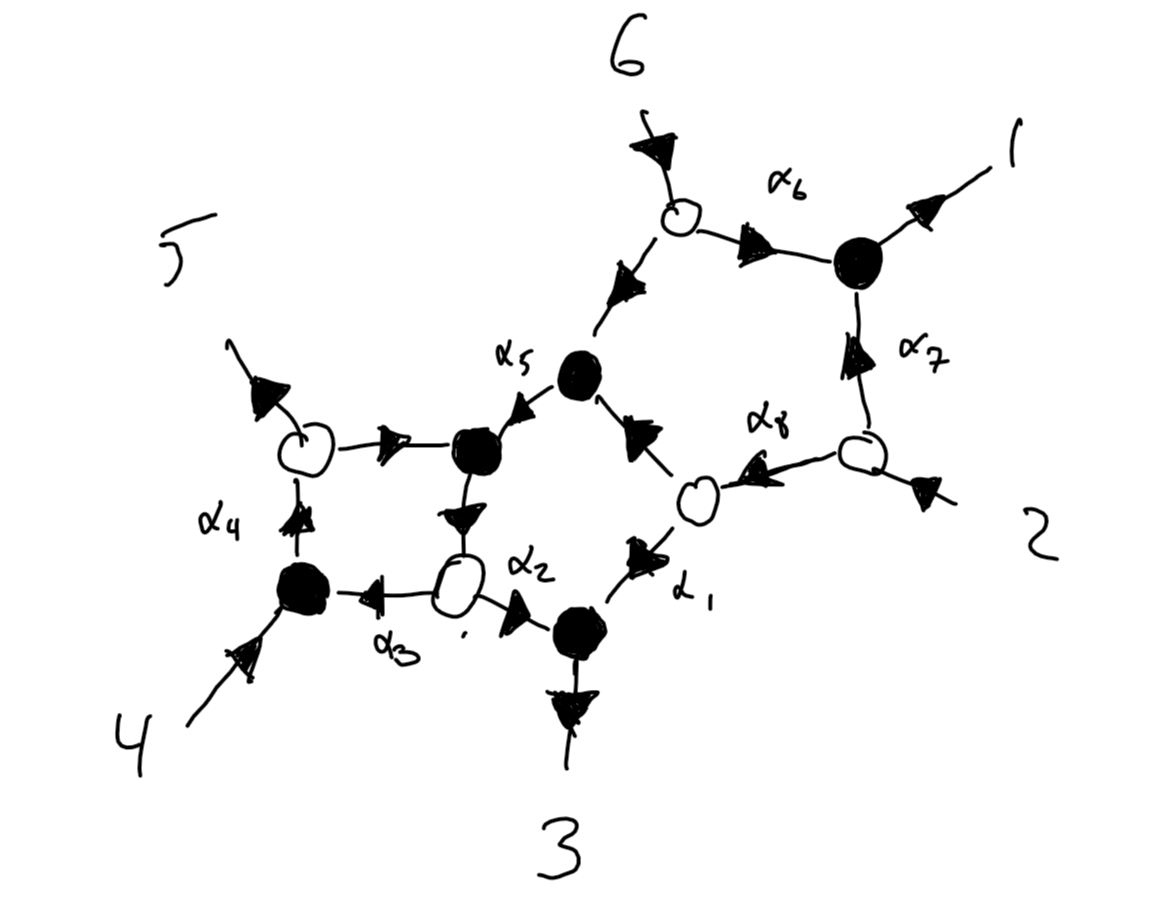
\includegraphics[width=0.4\linewidth]{3+5L}
	\caption{5+3 six-point NMHV diagram with internal cycle. To calculate the form of the cut, the same diagram with the cycle reversed also contributes.}
	\label{fig:5pt3l}
\end{figure}\noindent 
Where another diagram with the internal cycle is reversed also contributes to the form of the cut. The edge-variables are found to be
\begin{equation}
	\begin{aligned}
		& \alpha_1 = \frac{\sab{612}}{\aMs{6}{Q_{612}}{3}}\,, \quad \alpha_2 = \frac{[45]}{[34]}\,, \quad \alpha_3 = \frac{[45]\aMs{2}{Q_{612}}{3}}{[34]\aMs{2}{Q_{612}}{4}}\,, \quad \alpha_4 = -\frac{\aMs{2}{Q_{612}}{4}}{\aMs{2}{Q_{612}}{5}}\,,\\ 
		&\alpha_5 = \frac{\aMs{2}{Q_{612}}{4}}{\ab{62}[45]}\,, 
		\quad
		\alpha_6 = \frac{\ab{12}}{\ab{62}}\,,\quad \alpha_7 = \frac{\ab{61}}{\ab{62}}\,,\quad
		\alpha_8 = - \frac{\aMs{6}{Q_{612}}{3}}{\aMs{2}{Q_{612}}{3}}\,.
	\end{aligned}
\end{equation}
The Jacobian from solving the delta functions is $ \frac{\ab{26}\sqb{35}^4\aMs{2}{Q_{612}}{4}}{\sqb{34}^3\aMs{2}{Q_{612}}{5}^2\aMs{2}{Q_{612}}{3}}$ while the internal cycle Jacobian is
\begin{equation}
	\begin{aligned}
		J_a=\frac{\aMs{2}{Q_{612}}{4}\sqb{35}}{\aMs{2}{Q_{612}}{5}\sqb{34}}
	\end{aligned}
\end{equation}
Using the approach described at five-point we can infer the Jacobian of the diagam with opposite cycle to be
\begin{equation}
	\begin{aligned}
		J_b=\frac{\aMs{2}{Q_{612}}{4}\sqb{35}}{\aMs{2}{Q_{612}}{3}\sqb{45}}
	\end{aligned}
\end{equation}
The form is then
\begin{equation}
	\begin{aligned}
		\dd\Omega&=\frac{\ab{26}^4\sqb{24}^4\delta(P)}{s_{612}\ab{12}\ab{16}\sqb{34}\sqb{45}\aMs{2}{Q_{612}}{5}\aMs{6}{Q_{612}}{3}}\left[\left(\frac{\aMs{2}{Q_{612}}{4}\sqb{35}}{\aMs{2}{Q_{612}}{5}\sqb{34}}\right)^{-4}+\left(\frac{\aMs{2}{Q_{612}}{4}\sqb{35}}{\aMs{2}{Q_{612}}{3}\sqb{45}}\right)^{-4}\right]
	\end{aligned}
\end{equation}
Let us further examine the six-point NMHV case by looking at an example of a 4+4 diagram. It is not possible to orient the graph with a closed cycle for the external helicity configuration of $(1^+,2^-,3^+,4^-,5^+,6^-)$, so instead we consider the following two diagrams.
\begin{figure}[H]
	\centering
	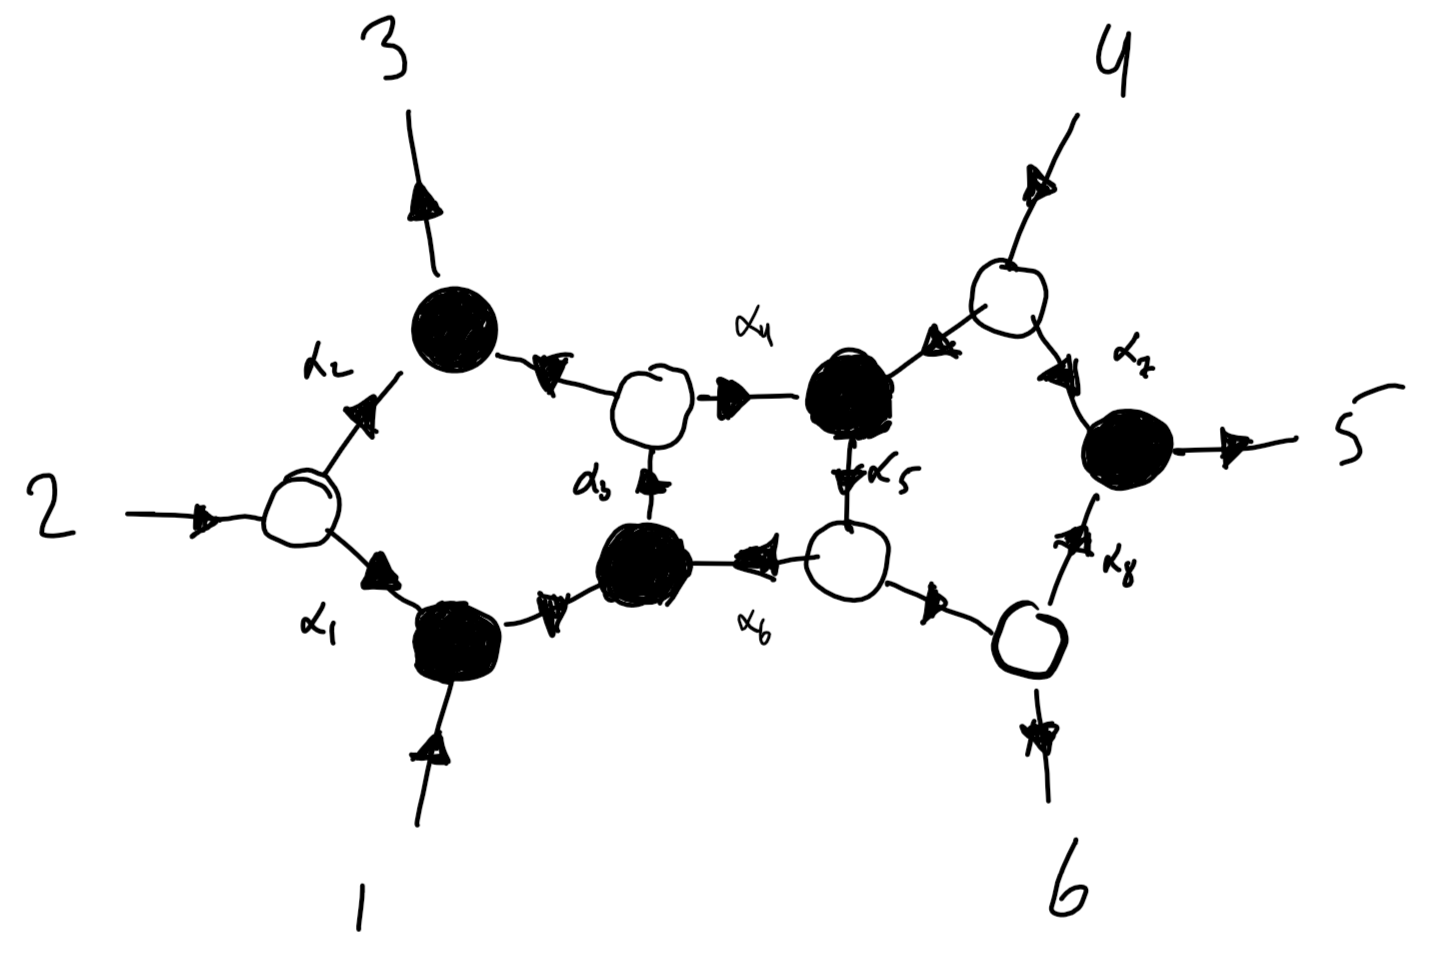
\includegraphics[width=0.9\linewidth]{6pt}
	\caption{All six point NMHV diagrams for the specific helicity configuration}
	\label{fig:two-loop}
\end{figure}
\noindent They are the only ones that arise when fixing the internal states as shown. Here we explicitly show the $C_A$-matrices
\begin{equation}
	\begin{aligned}
		C_A&=\left(
		\begin{array}{cccccc}
			1 & 0 & \alpha _3 \delta_a & 0 & \alpha _3 \alpha _4 \alpha _5 \alpha _8 \delta_a & \alpha _3 \alpha _4 \alpha _5 \delta_a \\
			0 & 1 & \alpha _1 \alpha _3 \delta_a+\alpha _2 & 0 & \alpha _1 \alpha _3 \alpha _4 \alpha _5 \alpha _8 \delta_a & \alpha _1 \alpha _3 \alpha _4 \alpha _5 \delta_a \\
			0 & 0 & \alpha _3 \alpha _5 \alpha _6 \delta_a & 1 & \alpha _5 \alpha _8 \delta_a+\alpha _7 & \alpha _5 \delta_a
		\end{array}
		\right)\\
		C_A^{\perp}&=\left(
		\begin{array}{cccccc}
			-\alpha _3 \delta_a & -\alpha _1 \alpha _3 \delta_a-\alpha _2 & 1 & -\alpha _3 \alpha _5 \alpha _6 \delta_a & 0 & 0 \\
			-\alpha _3 \alpha _4 \alpha _5 \alpha _8 \delta_a & -\alpha _1 \alpha _3 \alpha _4 \alpha _5 \alpha _8 \delta_a & 0 & -\alpha _5 \alpha _8 \delta_a-\alpha _7 & 1 & 0 \\
			-\alpha _3 \alpha _4 \alpha _5 \delta_a & -\alpha _1 \alpha _3 \alpha _4 \alpha _5 \delta_a & 0 & -\alpha _5 \delta_a & 0 & 1 \\
		\end{array}
		\right)
	\end{aligned}
\end{equation}
The edge-variables for diagram $A$ are found to be
\begin{align*}
 \alpha_1 = \frac{[23]}{[13]}\,, \quad \alpha_2 =- \frac{[12]}{[13]}&\,,~~
	\alpha_3 = - \frac{\aMs{6}{Q_{456}}{1}}{\aMs{6}{Q_{456}}{3}}, \quad
	\alpha_4 = \frac{\ab{46}\sqb{13}}{\aMs{6}{Q_{456}}{1}}\,,\\
	 \alpha_5 = \frac{\aMs{6}{Q_{456}}{1}}{\aMs{4}{Q_{456}}{1}}\,,\quad
	 \,\alpha_6 &= \frac{\sab{456}}{\aMs{6}{Q_{456}}{1}}\,, \quad \alpha_7 = \frac{\ab{56}}{\ab{46}}\,, \quad
	\alpha_8 = \frac{\ab{45}}{\ab{46}}\,  
\end{align*}
with a factor of $\frac{\ab{46}^3\ab{13}^3}{\aMs{4}{Q_{456}}{1}^2\aMs{6}{Q_{456}}{3}^2}$ from solving the delta functions and a Jacobian of
\begin{equation}
	\begin{aligned}
		J_a=\delta_a^{-1}=\frac{\aMs{4}{Q_{456}}{3}\aMs{6}{Q_{456}}{1}}{\aMs{4}{Q_{456}}{1}\aMs{6}{Q_{456}}{3}}
	\end{aligned}
\end{equation}
Using the aforementioned we can also infer the Jacobian of the diagram with the internal cycle reversed
\begin{equation}
	\begin{aligned}
		J_b=\frac{\aMs{4}{Q_{456}}{3}\aMs{6}{Q_{456}}{1}}{[13]\ab{46}s_{456}}
	\end{aligned}
\end{equation}
The form obtained
is then
\begin{equation}
	\begin{aligned} \label{eq:6pt}
		\dd\Omega&=\frac{\ab{46}^4\sqb{13}^4}{s_{456}\ab{45}\ab{56}\sqb{12}\sqb{23}\aMs{4}{Q_{456}}{1}\aMs{6}{Q_{456}}{3}}\left(
		\left[\frac{\aMs{4}{Q_{456}}{3}\aMs{6}{Q_{456}}{1}}{\aMs{4}{Q_{456}}{1}\aMs{6}{Q_{456}}{3}}\right]^{-4}+\left[\frac{\aMs{4}{Q_{456}}{3}\aMs{6}{Q_{456}}{1}}{[13]\ab{46}s_{456}}\right]^{-4}
		\right)	
	\end{aligned}
\end{equation}
We will now analyze the singularity structure of this diagram, by assigning loop momenta to the three loops and putting the internal propagators on-shell.
\subsection{Singularities}
To find the singularity structure of the form obtained, we first assign the three loop momenta $\ell_1,\ell_2$, and $\ell_3$, in the following way
\begin{figure}[H]
	\centering
	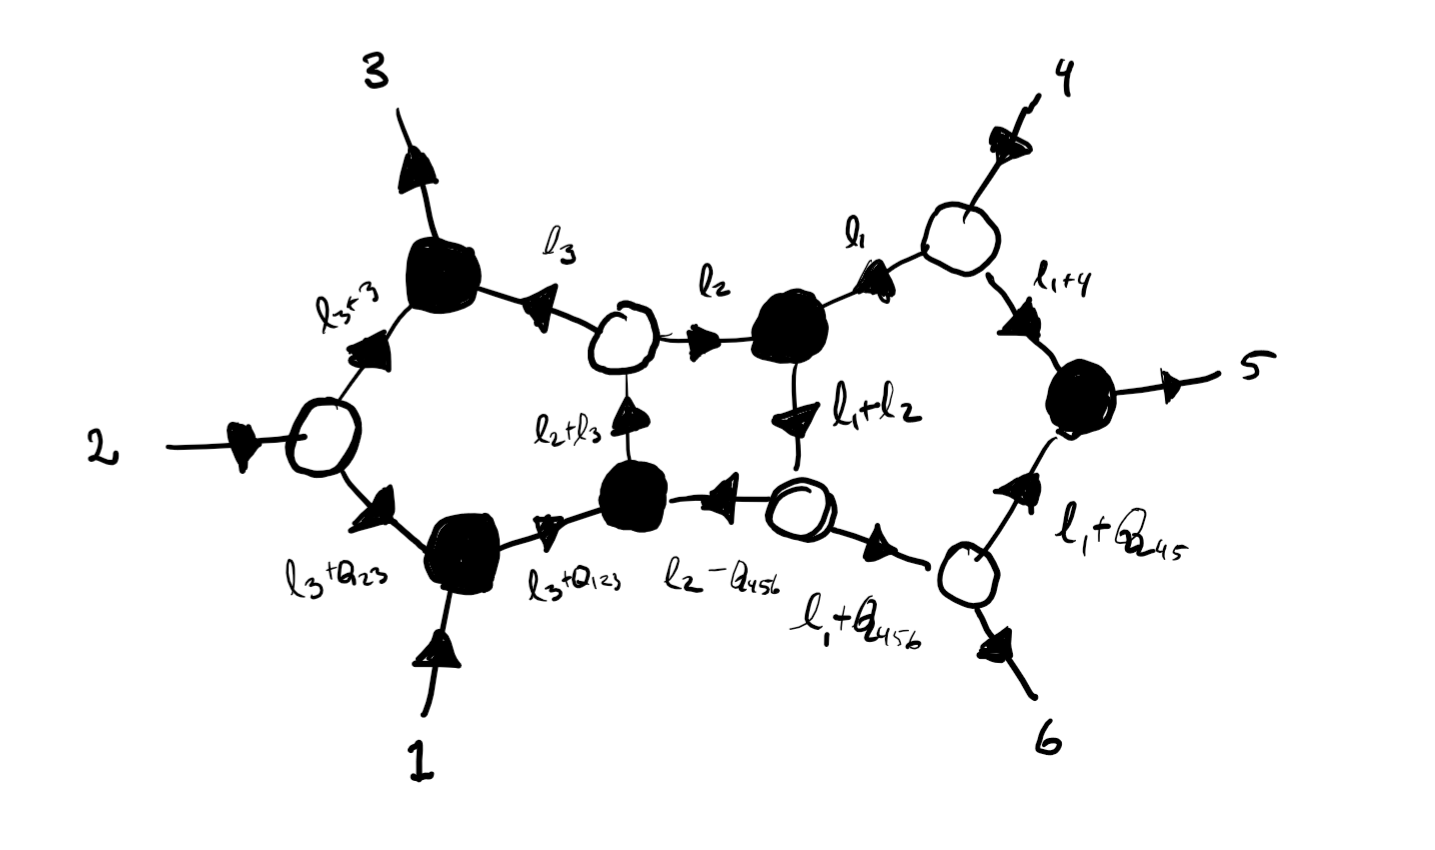
\includegraphics[width=0.5\linewidth]{sing}
	\caption{Six point NMHV 4+4 diagram with assigned loop momenta}
	\label{fig:two-loop}
\end{figure}
\noindent We then put the internal propagators on shell, which gives the following solutions for the internal momenta
%\begin{equation}
%	\begin{aligned}
%	\ell_1=\frac{\tilde\lambda_4}{\ab{46}}\aMs{6}{Q_{456}}{\bm\cdot},~~~~~~\ell_2=\frac{1}{\green{\aMs{6 }{Q_{456}}{1}}}\aMs{6 }{Q_{456}}{\bm\cdot}\aMs{\bm \cdot }{Q_{456}}{1},~~~~~~	\ell_3=\frac{\tilde\lambda_3}{\sqb{13}}\aMs{\bm\cdot}{Q_{456}}{1},\\
%	\ell_1+4=\frac{\textcolor{yellow}{\ab{56}}}{\ab{46}}\lambda_4\tilde{\lambda}_5,~~~~~~\ell_2+\ell_3=\frac{\aMs{6 }{Q_{456}}{3}}{\green{\aMs{6 }{Q_{456}}{1}}}\aMs{\bm \cdot }{Q_{456}}{1}\frac{\tilde\lambda_4}{\sqb{13}},~~~~~~\ell_3+3=-\frac{\blue{\sqb{12}}}{\sqb{13}}\lambda_2\tilde{\lambda}_3,
%	\\
%	\ell_1+Q_{45}=\frac{\textcolor{purple}{\ab{45}}}{\ab{46}}\lambda_6\tilde{\lambda}_4,~~~~~~\ell_2-Q_{456}=\frac{\orange{s_{456}}}{\green{\aMs{6 }{Q_{456}}{1}}}\lambda_3\tilde\lambda_4,~~~~~~\ell_3+Q_{23}=\frac{\red{\sqb{23}}}{\sqb{13}}\lambda_2\tilde{\lambda}_1,\\
%	\ell_1+Q_{456}=\frac{\lambda_6}{\ab{46}}\aMs{4}{s_{456}}{\bm \cdot},~~~~~~\ell_1+\ell_2=\frac{\aMs{4 }{Q_{456}}{1}}{\green{\aMs{6 }{Q_{456}}{1}}}\aMs{6 }{Q_{456}}{\bm \cdot}\frac{\lambda_6}{\ab{46}},~~~~~~\ell_3+Q_{123}=\frac{\tilde\lambda_1}{\sqb{13}}\aMs{\bm\cdot}{s_{456}}{3},
%	\end{aligned}
%\end{equation}
\begin{equation}
	\begin{aligned}
		\ell_1=\frac{\tilde\lambda_4}{\pink{\ab{46}}}\aMs{6}{Q_{456}}{\bm\cdot},~~~~~~\ell_2=\frac{1}{\green{\aMs{6 }{Q_{456}}{1}}}\aMs{6 }{Q_{456}}{\bm\cdot}\aMs{\bm \cdot }{Q_{456}}{1},~~~~~~	\ell_3=\frac{\tilde\lambda_3}{\brown{\sqb{13}}}\aMs{\bm\cdot}{Q_{456}}{1},\\
		\ell_1+4=\frac{\textcolor{yellow}{\ab{56}}}{\pink{\ab{46}}}\lambda_4\tilde{\lambda}_5,~~~~~~\ell_2+\ell_3=\frac{\aMs{6 }{Q_{456}}{3}}{\green{\aMs{6 }{Q_{456}}{1}}}\aMs{\bm \cdot }{Q_{456}}{1}\frac{\tilde\lambda_4}{\brown{\sqb{13}}},~~~~~~\ell_3+3=-\frac{\blue{\sqb{12}}}{\brown{\sqb{13}}}\lambda_2\tilde{\lambda}_3,
		\\
		\ell_1+Q_{45}=\frac{\textcolor{purple}{\ab{45}}}{\pink{\ab{46}}}\lambda_6\tilde{\lambda}_4,~~~~~~\ell_2-Q_{456}=\frac{\orange{s_{456}}}{\green{\aMs{6 }{Q_{456}}{1}}}\lambda_3\tilde\lambda_4,~~~~~~\ell_3+Q_{23}=\frac{\red{\sqb{23}}}{\brown{\sqb{13}}}\lambda_2\tilde{\lambda}_1,\\
		\ell_1+Q_{456}=\frac{\lambda_6}{\pink{\ab{46}}}\aMs{4}{s_{456}}{\bm \cdot},~~~~~~\ell_1+\ell_2=\frac{\aMs{4 }{Q_{456}}{1}}{\green{\aMs{6 }{Q_{456}}{1}}}\aMs{6 }{Q_{456}}{\bm \cdot}\frac{\lambda_6}{\pink{\ab{46}}},~~~~~~\ell_3+Q_{123}=\frac{\tilde\lambda_1}{\brown{\sqb{13}}}\aMs{\bm\cdot}{s_{456}}{3},
	\end{aligned}
\end{equation}
Comparing this with the edge-variables, we have highlighted some of the common factors among them. 
\begin{align*}
	\alpha_1 = \frac{\red{[23]}}{\brown{[13]}}\,, \quad \alpha_2 = -\frac{\blue{[12]}}{\brown{[13]}}&\,,~~
	\alpha_3 = - \frac{\green{\aMs{6}{Q_{456}}{1}}}{\aMs{6}{Q_{456}}{3}}, \quad
	\alpha_4 =  \frac{\pink{\ab{46}}\brown{[13]}}{\green{\aMs{6}{Q_{456}}{1}}}\,,\\
	\alpha_5 = \frac{\green{\aMs{6}{Q_{456}}{1}}}{\aMs{4}{Q_{456}}{1}}\,,\quad
	\,\alpha_6 &= \frac{\orange{\sab{456}}}{\green{\aMs{6}{Q_{456}}{1}}}\,, \quad \alpha_7 = \frac{\textcolor{yellow}{\ab{56}}}{\pink{\ab{46}}}\,, \quad
	\alpha_8 = \frac{\textcolor{purple}{\ab{45}}}{\pink{\ab{46}}}\,  
\end{align*}
We see that sending $\{\alpha_1,\alpha_2,\alpha_6,\alpha_7,\alpha_8\}\to 0$ erases the corresponding edge, while the same happens by sending $\{\alpha_3,\alpha_5\}\to \infty$.
Further we can identify
\begin{equation}
	\begin{aligned}
		\ell_1\to& \infty,~~~~\text{ for }\pink{ \ab{46}}\to 0,\\
		\ell_2\to& \infty,~~~~\text{ for } \green{\aMs{6}{Q_{456}}{1}}\to 0,\\
		\ell_3\to& \infty,~~~~\text{ for } \brown{\sqb{13}}\to 0.\\
	\end{aligned}
\end{equation}
We see that in the final form \eqref{eq:6pt}, these will contribute as higher order poles stemming from the Jacobian factors.  From these equations we also see that erasing $\alpha_4$ either comes from sending $\sqb{13}$ or $\ab{46}$ to 0 (which would send $\ell_1$ or $\ell_3$ to $\infty$) or from sending $\aMs{6}{Q_{456}}{1}\to \infty$, which would erase $\alpha_3,\alpha_5,$ and $\alpha_6$ as well.

Finally we will in the next section discuss how to construct higher loop, or non-reduced, on-shell diagrams. 
\newpage
\section{Higher loops\label{sec:higherloops}}
One can get to higher loops with the same number of points by attaching two connected vertices to one of the graphs we have already considered. We will do this at four point to show how the form is constructed and then proceed to analyze one five-point three-loop diagram with no internal cycles and one with an internal cycle. Finally we analyze the singularity structure by comparing with the solution obtained by explicitly solving the on-shell constraints of the internal momenta.
\subsection{2 loop four-point}
At four points we can attach the two connected vertices to the four point diagram from section \ref{sec:on-she-intro} to make the following two-loop diagram, with corresponding C-matrix
\begin{figure}[H]
	\centering
	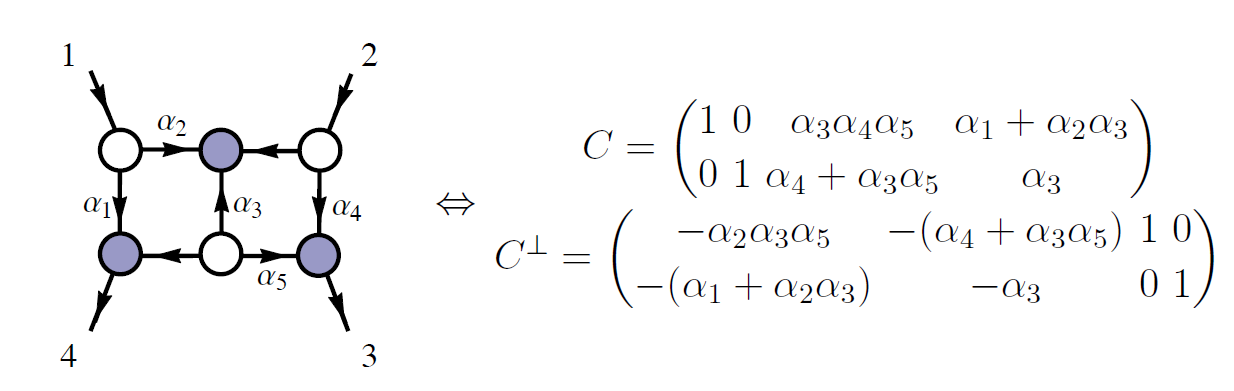
\includegraphics[width=0.7\linewidth]{two-loop}
	\caption{}
	\label{fig:two-loop}
\end{figure}
\noindent Solving the bosonic delta-functions one obtains the following equations
\begin{equation}
	\begin{aligned}
		0&=\alpha_{4} \langle 1 2 \rangle + \alpha_{3} \alpha_{5} \langle 1 2 \rangle - \langle 1 3 \rangle
		&&0=\alpha_{2} \alpha_{3} \alpha_{5} \langle 1 2 \rangle - \langle 2 3 \rangle
		\\
		0&=\alpha_{3} \langle 1 2 \rangle - \langle 1 4 \rangle
		&&0=-((\alpha_{1} + \alpha_{2} \alpha_{3}) \langle 1 2 \rangle) - \langle 2 4 \rangle
		\\
	\end{aligned}
\end{equation}
Then, taking $\alpha_4$ as the free parameter, we find
\begin{equation}
	\begin{aligned}
		\alpha_1=-\frac{\alpha_4\ab{24}-\ab{34}}{\alpha_4\ab{12}-\ab{13}},~~~~\alpha_2=\frac{\ab{23}}{\alpha_4\ab{12}-\ab{13}},~~~~\alpha_3=\frac{\ab{14}}{\ab{12}},~~~~\alpha_5=-\frac{\alpha_4\ab{12}-\ab{13}}{\ab{14}},~~~~
	\end{aligned}
\end{equation}
So that the $\mathcal{N}=0$ form, after multiplying by the delta function Jacobian $\frac{\ab{12}^2}{\ab{14}\left(\alpha_4\ab{12}-\ab{13}\right)}$, is
\begin{equation}
	\begin{aligned}
	\dd\Omega = \frac{\ab{12}^4}{\alpha_4\ab{12}\ab{23}\ab{41}\left(\alpha_4\ab{24}-\ab{34}\right)}\delta(P)	\end{aligned}
\end{equation}
Before we approach a diagram with an internal cycle, we will first give another example of a higher loop diagram, specifically at five points.
\subsection{Three loop five-point in $\mathcal{N}=0$, no internal cycle}
Just like in the four-point example we can add a connected pair of vertices to one of the five point diagrams, to get a three loop graph. An example of such a graph is shown below
\begin{figure}[H]
	\centering
	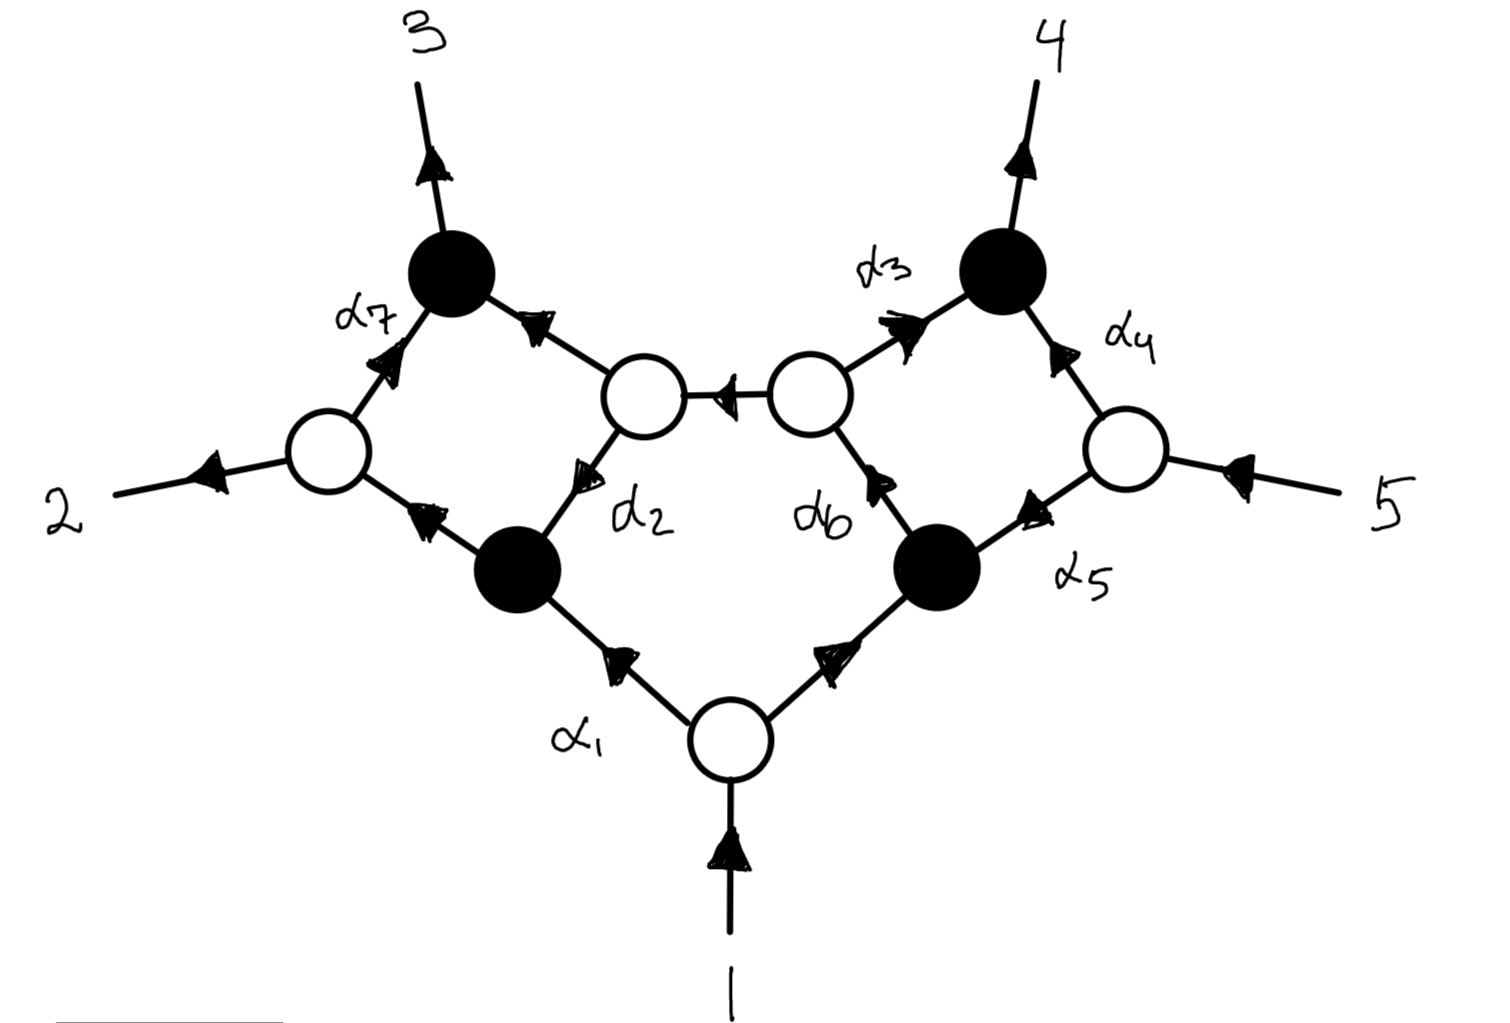
\includegraphics[width=0.5\linewidth]{5pt3l}
	\caption{Three loop five-point diagram with no cycles}
	\label{fig:5pt3l_1}
\end{figure}
\noindent The on-shell condition imposed on the three loop momenta leaves us with $3\times 4-11=1$ unfixed parameter. The C-matrices are
\begin{equation}
	\begin{aligned}
		C&=\left(
		\begin{array}{ccccc}
			1 & \alpha _1+\alpha _2 \alpha _6 & \alpha _2 \alpha _7 \alpha _6+\alpha _6+\alpha _1 \alpha _7 & \alpha _3 \alpha _6 & 0 \\
			0 & \alpha _2 \alpha _5 \alpha _6 & \alpha _5 \alpha _6 \left(\alpha _2 \alpha _7+1\right) & \alpha _4+\alpha _3 \alpha _5 \alpha _6 & 1 \\
		\end{array}
		\right)\\
		C_\perp&=\left(
		\begin{array}{ccccc}
			-\alpha _1-\alpha _2 \alpha _6 & 1 & 0 & 0 & -\alpha _2 \alpha _5 \alpha _6 \\
			-\alpha _6-\left(\alpha _1+\alpha _2 \alpha _6\right) \alpha _7 & 0 & 1 & 0 & -\alpha _5 \alpha _6 \left(\alpha _2 \alpha _7+1\right) \\
			-\alpha _3 \alpha _6 & 0 & 0 & 1 & -\alpha _4-\alpha _3 \alpha _5 \alpha _6 \\
		\end{array}
		\right)
	\end{aligned}
\end{equation}
With the following corresponding equations stemming from the delta function
\begin{equation}
	\begin{aligned}
		\delta(C_\perp\cdot \lambda)&\rightarrow\begin{cases}
	0&=-\langle 1 2 \rangle + \alpha_{2} \alpha_{5} \alpha_{6} \langle 1 5 \rangle
		\\
		0&=-((\alpha_{1} + \alpha_{2} \alpha_{6}) \langle 1 5 \rangle) + \langle 2 5 \rangle
		\\
		0&=-\langle 1 3 \rangle + \alpha_{5} \alpha_{6} (1 + \alpha_{2} \alpha_{7}) \langle 1 5 \rangle
		\\
		0&=-((\alpha_{6} + \alpha_{1} \alpha_{7} + \alpha_{2} \alpha_{6} \alpha_{7}) \langle 1 5 \rangle) + \langle 3 5 \rangle
		\\
		0&=-\langle 1 4 \rangle + (\alpha_{4} + \alpha_{3} \alpha_{5} \alpha_{6}) \langle 1 5 \rangle
		\\
		0&=-(\alpha_{3} \alpha_{6} \langle 1 5 \rangle) + \langle 4 5 \rangle
		\end{cases}
%			\\
%		\delta(C_\perp\cdot \lambda)&\rightarrow
%		\begin{cases}
%		0&=\left[ 1 2 \right] - (\alpha_{6} + \alpha_{1} \alpha_{7} + \alpha_{2} \alpha_{6} \alpha_{7}) \left[ 2 3 \right] - \alpha_{3} \alpha_{6} \left[ 2 4 \right]
%		\\
%		0&=\left[ 1 3 \right] + (\alpha_{1} + \alpha_{2} \alpha_{6}) \left[ 2 3 \right] - \alpha_{3} \alpha_{6} \left[ 3 4 \right]
%		\\
%		0&=\left[ 1 4 \right] + (\alpha_{1} + \alpha_{2} \alpha_{6}) \left[ 2 4 \right] + (\alpha_{6} + \alpha_{1} \alpha_{7} + \alpha_{2} \alpha_{6} \alpha_{7}) \left[ 3 4 \right]
%		\\
%		0&=-(\alpha_{5} \alpha_{6} (1 + \alpha_{2} \alpha_{7}) \left[ 2 3 \right]) - (\alpha_{4} + \alpha_{3} \alpha_{5} \alpha_{6}) \left[ 2 4 \right] - \left[ 2 5 \right]
%		\\
%		0&=\alpha_{2} \alpha_{5} \alpha_{6} \left[ 2 3 \right] - (\alpha_{4} + \alpha_{3} \alpha_{5} \alpha_{6}) \left[ 3 4 \right] - \left[ 3 5 \right]
%		\\
%		0&=\alpha_{2} \alpha_{5} \alpha_{6} \left[ 2 4 \right] + \alpha_{5} \alpha_{6} (1 + \alpha_{2} \alpha_{7}) \left[ 3 4 \right] - \left[ 4 5 \right]
%	\end{cases}
	\end{aligned}
\end{equation}
%%%%%%%%%%%%%%
%
%
%
%
%
%
%
%
%
%
%
%
It is natural choice in this case to take either $\alpha_7$ or $\alpha_4$ as the free parameters. We take $\alpha_7$ and note that since removing $\alpha_7$ gives us one of the five-point graphs analyzed earlier in this report, one would expect the residue at $\alpha_7=0$ of the resulting form to match the five-point two loop result. Solving the delta-functions we find
\begin{equation}
	\begin{aligned}
\alpha_1&=-\frac{\ab{23}}{\alpha_7\ab{12}-\ab{13}},~~~~~~
\alpha_2=-\frac{\ab{12}}{\alpha_7\ab{12}-\ab{13}},~~~~~~
\alpha_3=-\frac{\ab{45}}{\alpha_7\ab{25}-\ab{35}}\\
\alpha_4&=-\frac{\alpha_7\ab{24}-\ab{34}}{\alpha_7\ab{25}-\ab{35}}
,~~~~~~
\alpha_5=\frac{\alpha_7\ab{12}-\ab{13}}{\alpha_7\ab{25}-\ab{35}}
,~~~~~~~~\,
\alpha_6=-\frac{\alpha_7\ab{25}-\ab{35}}{\ab{15}}
	\end{aligned}
\end{equation}
Such that
\begin{equation}
	\begin{aligned}
		&\delta(C_\perp\cdot \lambda)\delta(C\cdot\tilde \lambda)\\
		=&
		\frac{\ab{15}^3}{\left(\alpha_7\ab{12}-\ab{13}\right)
	\left(-\alpha_7\ab{25}+\ab{35}\right)^2	
	}\delta^4( P)
		\delta\left(\alpha_1+\frac{\ab{23}}{\alpha_7\ab{12}-\ab{13}}\right)
		\delta\left(\alpha_2+\frac{\ab{12}}{\alpha_7\ab{12}-\ab{13}}\right)\\&
		\delta\left(\alpha_3+\frac{\ab{45}}{\alpha_7\ab{25}-\ab{35}}\right)
		\delta\left(\alpha_4+\frac{\alpha_7\ab{24}-\ab{34}}{\alpha_7\ab{25}-\ab{35}}\right)
		\delta\left(\alpha_5-\frac{\alpha_7\ab{12}-\ab{13}}{\alpha_7\ab{25}-\ab{35}}\right)
		\delta\left(\alpha_6+\frac{\alpha_7\ab{25}-\ab{35}}{\ab{15}}\right),
	\end{aligned}
\end{equation}
and we get the form
\begin{equation}
	\begin{aligned}
	\dd \Omega=	\frac{\ab{15}^4}{\alpha_7 \ab{12}\ab{23}\ab{45}\ab{15}\left(\alpha_7\ab{24}-\ab{34}\right)}.
	\end{aligned}
\end{equation}
Taking the residue of the form at $\alpha_7=0$ one recovers the standard YM Parke-Taylor tree-level amplitude, as expected.
\begin{equation}
	\begin{aligned}
		\dd \Omega=	\frac{\ab{15}^4}{ \ab{12}\ab{23}\ab{34}\ab{45}\ab{51}}
	\end{aligned}
\end{equation}
Further, we note that the form has one other pole at $\alpha_7=\frac{\ab{34}}{\ab{24}}$. Since we now have an intuition for the procedure, let us repeat this for a diagram with an internal cycle.
\subsection{Three loop five-point in $\mathcal{N}=0$ with internal cycle}
We will consider the following graph
\begin{figure}[H]
	\centering
	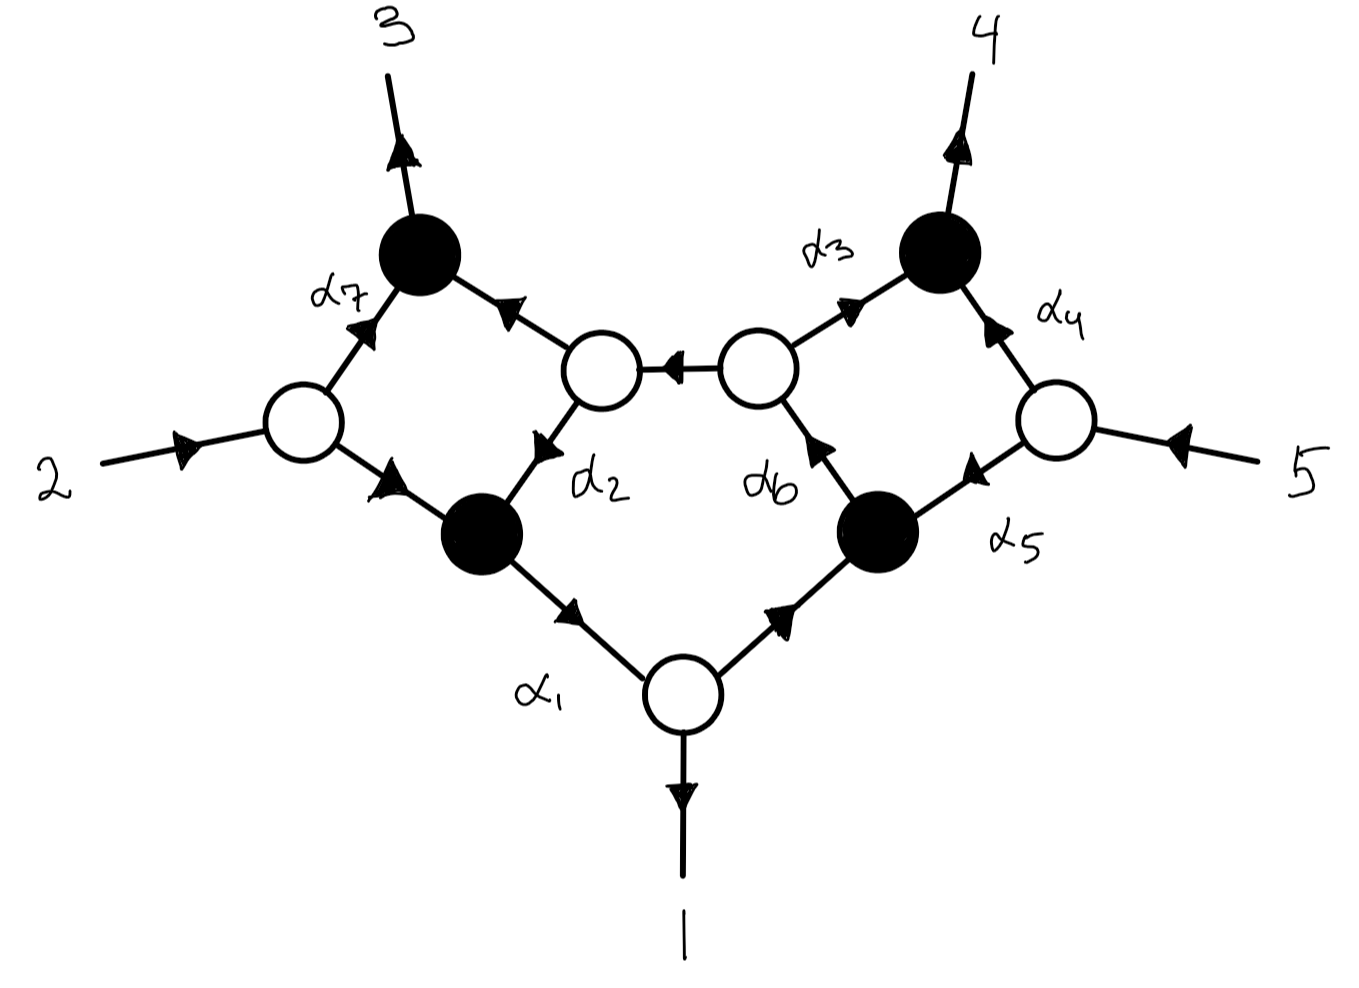
\includegraphics[width=0.5\linewidth]{5pt3l_2}
	\caption{Diagram $A$: three loop, five point}
	\label{fig:5pt3l_3}
\end{figure}
To get form of the cut, one has to fix the helicity configuration and then find all the configurations of the internal momenta that yield a perfect orientation. The only other possible diagram would have the internal cycle going clockwise instead; we will refer to that as diagram $B$. Since the bare form is the same for both diagrams, the only point of difference is the Jacobians. 

For diagram A, the C-matrices are
\begin{equation}
	\begin{aligned}
		C
		&=\left(
		\begin{array}{ccccc}
			\alpha _1 \delta_a & 1 & \alpha _1 \alpha _6 \delta_a+\alpha _7 & \alpha _1 \alpha _3 \alpha _6 \delta_a & 0 \\
			\alpha _1 \alpha _2 \alpha _5 \alpha _6 \delta_a & 0 & \alpha _5 \alpha _6 \delta_a & \alpha _3 \alpha _5 \alpha _6 \delta_a+\alpha _4 & 1 \\
		\end{array}
		\right)\\
		C_\perp&=
		\left(
		\begin{array}{ccccc}
			1 & -\alpha _1\delta_a & 0 & 0 & -\alpha _1 \alpha _2 \alpha _5 \alpha _6 \delta_a \\
0 & -\alpha _1 \alpha _6 \delta_a-\alpha _7 & 1 & 0 & -\alpha _5 \alpha _6 \delta_a \\
0 & -\alpha _1 \alpha _3 \alpha _6 \delta_a & 0 & 1 & -\alpha _3 \alpha _5 \alpha _6 \delta_a-\alpha _4 \\
		\end{array}
		\right),
	\end{aligned}
\end{equation}
where $\delta_a=\frac{1}{1-\alpha_1\alpha_2\alpha_6}$. The first delta-function constraint gives us
\begin{equation}
	\begin{aligned}
				\delta^{6}(C_\perp\cdot \lambda)&\rightarrow\begin{cases} 0&=
		\langle 1 2 \rangle + \alpha_{1} \alpha_{2} \alpha_{5} \alpha_{6} \delta_a \langle 2 5 \rangle
		\\0&=
		\langle 1 5 \rangle - \alpha_{1} \delta_a \langle 2 5 \rangle
		\\0&=
		-\langle 2 3 \rangle + \alpha_{5} \alpha_{6} \delta_a \langle 2 5 \rangle
		\\0&=
		(-\alpha_{7} - \alpha_{1} \alpha_{6} \delta_a) \langle 2 5 \rangle + \langle 3 5 \rangle
		\\0&=
		-\langle 2 4 \rangle - (-\alpha_{4} - \alpha_{3} \alpha_{5} \alpha_{6} \delta_a) \langle 2 5 \rangle
		\\0&=
		-(\alpha_{1} \alpha_{3} \alpha_{6} \delta_a \langle 2 5 \rangle) + \langle 4 5 \rangle
				\end{cases}
	\end{aligned}
\end{equation}
Solving the delta-functions we find
\begin{equation}
	\begin{aligned}
		\alpha_1&=-\frac{
			\alpha_7\ab{12}-\ab{13}
		}{	\ab{23}},~~~~~~
		\alpha_2=-\frac{\ab{12}}{\alpha_7\ab{12}-\ab{13}},~~~~~~
		\alpha_3=-\frac{\ab{45}}{\alpha_7\ab{25}-\ab{35}}\\
		\alpha_4&=-\frac{\alpha_7\ab{24}-\ab{34}}{\alpha_7\ab{25}-\ab{35}}
		,~~~~~~
		\alpha_5=\frac{\alpha_7\ab{12}-\ab{13}}{\alpha_7\ab{25}-\ab{35}}
		,~~~~~~~~\,
		\alpha_6=-\frac{\alpha_7\ab{25}-\ab{35}}{\ab{15}}
		\\
		\delta_a&=-\frac{\ab{15}\ab{23}}{\ab{25}\left(\alpha_7\ab{12}-\ab{13}\right)}
	\end{aligned}
\end{equation}
\begin{equation}
	\begin{aligned}
		&\delta(C_\perp\cdot \lambda)\delta(C\cdot \tilde \lambda)\\
		=&
		\frac{\ab{15}^4\left(\alpha_7\ab{12}-\ab{13}\right)^{\phantom{2}}}{\ab{15}^2\ab{23}^2 \left(-\alpha_7\ab{25}+\ab{35}\right)^2}\delta^4( P)
		\delta\left(\alpha_1+\frac{
			\alpha_7\ab{12}-\ab{13}
		}{	\ab{23}}\right)
		\delta\left(\alpha_2+\frac{\ab{12}}{\alpha_7\ab{12}-\ab{13}}\right)\\&
		\delta\left(\alpha_3+\frac{\ab{45}}{\alpha_7\ab{25}-\ab{35}}\right)
		\delta\left(\alpha_4+\frac{\alpha_7\ab{24}-\ab{34}}{\alpha_7\ab{25}-\ab{35}}\right)
		\delta\left(\alpha_5-\frac{\alpha_7\ab{12}-\ab{13}}{\alpha_7\ab{25}-\ab{35}}\right)
		\delta\left(\alpha_6+\frac{\alpha_7\ab{25}-\ab{35}}{\ab{15}}\right)
	\end{aligned}
\end{equation}
The bare form matches that of our earlier diagram (albeit with a different helicity structure)
\begin{equation}
	\begin{aligned}
		\dd \Omega_{\text{bare}}=	\frac{\ab{25}^4}{\alpha_7 \ab{12}\ab{51}\ab{23}\ab{45}\left(\alpha_7\ab{24}-\ab{34}\right)}
	\end{aligned}
\end{equation}
and we note that taking the residue of the form at $\alpha_7=0$ one recovers the standard YM Parke-Taylor tree-level amplitude
\begin{equation}
	\begin{aligned}
			\frac{\ab{25}^4}{ \ab{12}\ab{23}\ab{34}\ab{45}\ab{51}}
	\end{aligned}
\end{equation}
To get the form of the cut we find that the Jacobian is
\begin{equation}
	\begin{aligned}
		J_a=\delta_a^{-1}=
		\frac{\ab{25}\left(\alpha_7\ab{12}-\ab{13}\right)}{\ab{15}\ab{23}}
	\end{aligned}
\end{equation}
While the Jacobian for the diagram with the internal cycle in the opposite direction is
\begin{equation}
	\begin{aligned}
		J_b=
		\frac{\ab{25}\left(\alpha_7\ab{12}-\ab{13}\right)}{\ab{12}\left(\alpha_7\ab{25}-\ab{35}\right)}
	\end{aligned}
\end{equation}
Which gives the total $\mathcal{N}=0$ form
\begin{equation}
	\begin{aligned}
		 \dd\Omega =\frac{\ab{25}^4}{\alpha_7 \ab{12}\ab{51}\ab{23}\ab{45}\left(\alpha_7\ab{24}-\ab{34}\right)}\left(	\left[\frac{\ab{25}\left(\alpha_7\ab{12}-\ab{13}\right)}{\ab{15}\ab{23}}\right]^{-4}+
		\left[\frac{\ab{25}\left(\alpha_7\ab{12}-\ab{13}\right)}{\ab{12}\left(\alpha_7\ab{25}-\ab{35}\right)}\right]^{-4}\right)
	\end{aligned}
\end{equation}
\subsection{Singularities}
To look at the singularity structure of the five-point three-loop on-shell diagram, we once again  look at 
\begin{figure}[H]
	\centering
	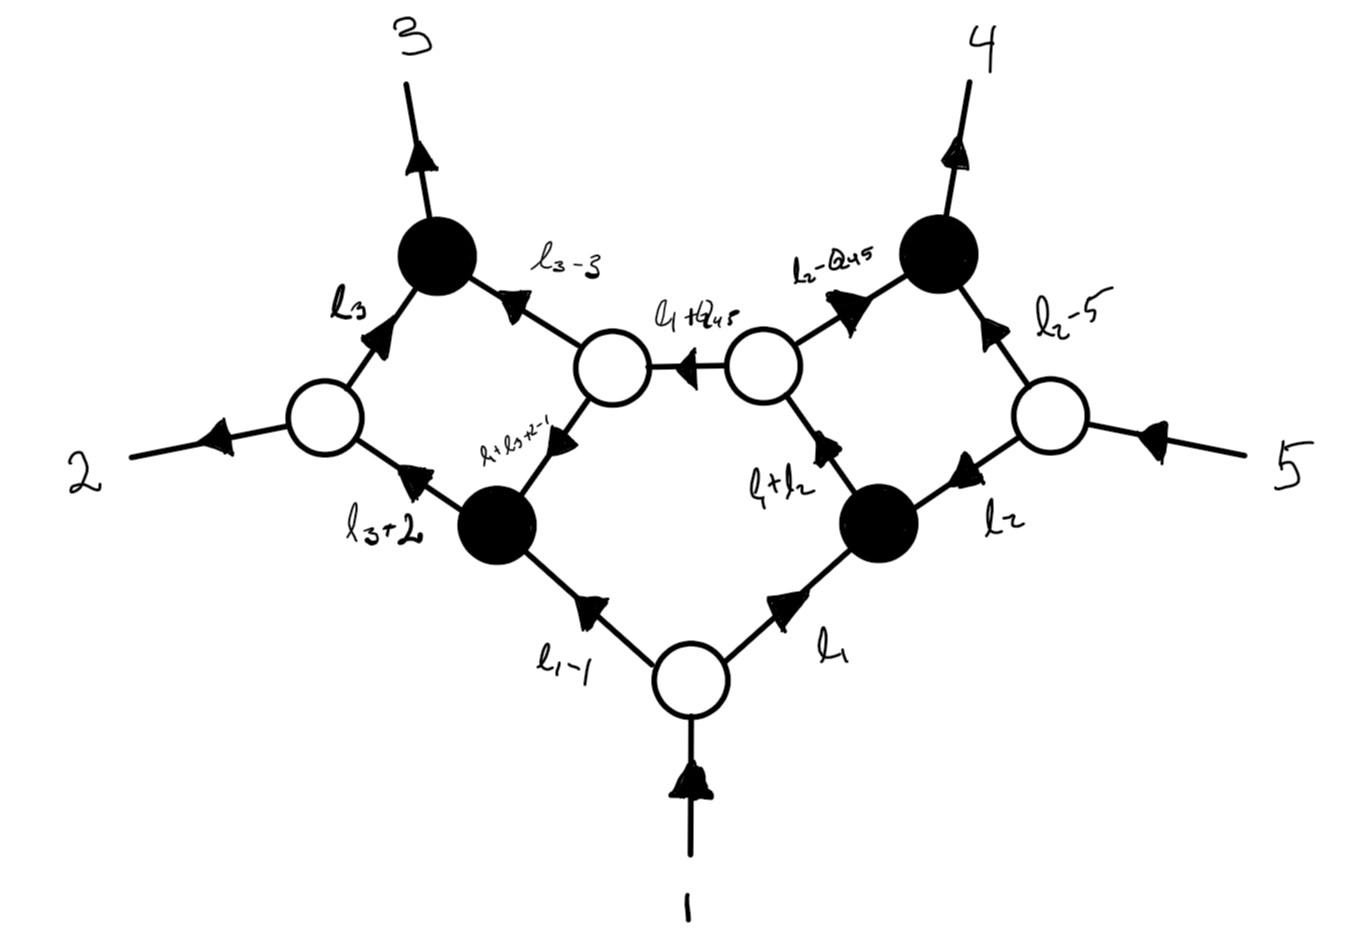
\includegraphics[width=0.5\linewidth]{5pt3l3}
	\caption{Three-loop diagram with loop momenta assigned.}
	\label{fig:5pt3l_2}
\end{figure}
\noindent Where we have assigned 3 different loop-momenta, $\ell_1$, $\ell_2$, and $\ell_3$. 
The momenta is found to be
\begin{equation}
	\begin{aligned}
\ell_3&=\textcolor{blue}{z} \lambda_2\tilde\lambda_3,~~~~~~
	\ell_3+2 = \lambda_2\left(z \tilde \lambda_3- \tilde \lambda_2\right)
,~~~~~~
	\ell_3-3 = \tilde \lambda_3\left(z  \lambda_2+ \lambda_3\right)\\
	\ell_1&=\frac{\lambda_1}{\green{z\ab{12}-\ab{13}}}\left(z\aMs{2}{Q_{123}}{\bm\cdot}-\aMs{3}{Q_{123}}{\bm\cdot}\right),~~~
	\ell_2=-\frac{\lambda_5}{\orange{z\ab{25}-\ab{35}}}\left(z\aMs{2}{Q_{123}}{\bm\cdot}-\aMs{3}{Q_{123}}{\bm\cdot}\right)
	\\
	\ell_2-5&=\frac{\textcolor{red}{z\ab{24}-\ab{34}}}{\orange{z\ab{25}-\ab{35}}}\lambda_5\tilde\lambda_4,~~~~\ell_2-Q_{45}=
	\frac{\textcolor{purple}{\ab{45}}}{\textcolor{orange}{z\ab{25}-\ab{35}}}\tilde\lambda_4\left(z\lambda_2-\lambda_3\right)\\
	\ell_1-1&=\frac{\brown{\ab{23}}}{\textcolor{ForestGreen}{z\ab{12}-\ab{13}}}\lambda_1\left(z\tilde \lambda_3+\tilde\lambda_2 \right),~~~
\ell_1+Q_{45}=\frac{z\lambda_2-\lambda_3}{\green{z\ab{12}-\ab{13}}}\left(\ab{12}\tilde \lambda_2+z\ab{12}\tilde \lambda_3-\ab{13}\tilde \lambda_3\right)	
	\end{aligned}
\end{equation}
\begin{equation}
	\begin{aligned}
		\ell_1+\ell_2&=
		\frac{\pink{\ab{15}}\left(z\lambda_2-\lambda_3\right)}{\green{\left(z\ab{12}-\ab{13}\right)}\orange{\left(z\ab{25}-\ab{35}\right)}}\left(z\aMs{2}{Q_{123}}{\bm\cdot}-\aMs{3}{Q_{123}}{\bm\cdot}\right)\\
		\ell_1+\ell_3+2-1&=\frac{\textcolor{yellow}{\ab{12}}}{\green{z\ab{13}-\ab{12}}}
		\left(z \lambda_2-\lambda_3\right)\left(z \tilde\lambda_3-\tilde \lambda_2\right)
	\end{aligned}
\end{equation}
First we note that after identifying $\textcolor{blue}{z=-\alpha_7}$ the $\mathcal{N}=4$ form found by combining three-point amplitudes using the momenta above, matches the results obtained in the previous sections
\begin{equation}
	\begin{aligned}
	\dd \Omega_5=\frac{\delta(P)\delta(Q)}{z \ab{12}\ab{23}\ab{45}\ab{51}\left(z\ab{24}+\ab{34}\right)}
	\end{aligned}
\end{equation}
Further we see that the $\ell_2-5$ coefficient directly corresponds to the $\alpha_4$ edge, and below we have highlighted the common factors.
\begin{equation}
	\begin{aligned}
		\alpha_1&=\textcolor{ForestGreen}{-\frac{\brown{\ab{23}}}{\alpha_7\ab{12}-\ab{13}}},~~~~~~
		\alpha_2=-\frac{\textcolor{yellow}{\ab{12}}}{\green{\alpha_7\ab{12}-\ab{13}}},~~~~~~
		\alpha_3=\textcolor{orange}{-\frac{\textcolor{purple}{\ab{45}}}{\alpha_7\ab{25}-\ab{35}}}\\
		\alpha_4&=-\frac{\textcolor{red}{\alpha_7\ab{24}-\ab{34}}}{\orange{\alpha_7\ab{25}-\ab{35}}}
		,~~~~~~
		\alpha_5=\frac{\green{\alpha_7\ab{12}-\ab{13}}}{\orange{\alpha_7\ab{25}-\ab{35}}}
		,~~~~~~~~\,
		\alpha_6=-\frac{\orange{\alpha_7\ab{25}-\ab{35}}}{\pink{\ab{15}}}
	\end{aligned}
\end{equation}
Comparing Figure \ref{fig:5pt3l_1} and Figure \ref{fig:5pt3l_3} with their respective edge-variables, one sees that flipping arrows inside the diagram inverts the corresponding edge-variable. Sending one of $\{\alpha_1,\alpha_2,\alpha_3,\alpha_4,\alpha_5\}\to 0$ sends the corresponding edge to zero, while $\alpha_6\to\infty $ erases that edge. This agrees with the statement found at six points that edges that contain an arrow from a white to a black vertex is erasable by sending $\alpha\to 0$ and from black to white by $\alpha\to \infty$.  Finally, sending $\ell_1\to \infty$ gives a higher order pole in the form for the cut.
\newpage
\section{Six-, seven-, eight-, and nine-point MHV results} 
At six and seven points we obtain
\begin{figure}[H]
	\centering
	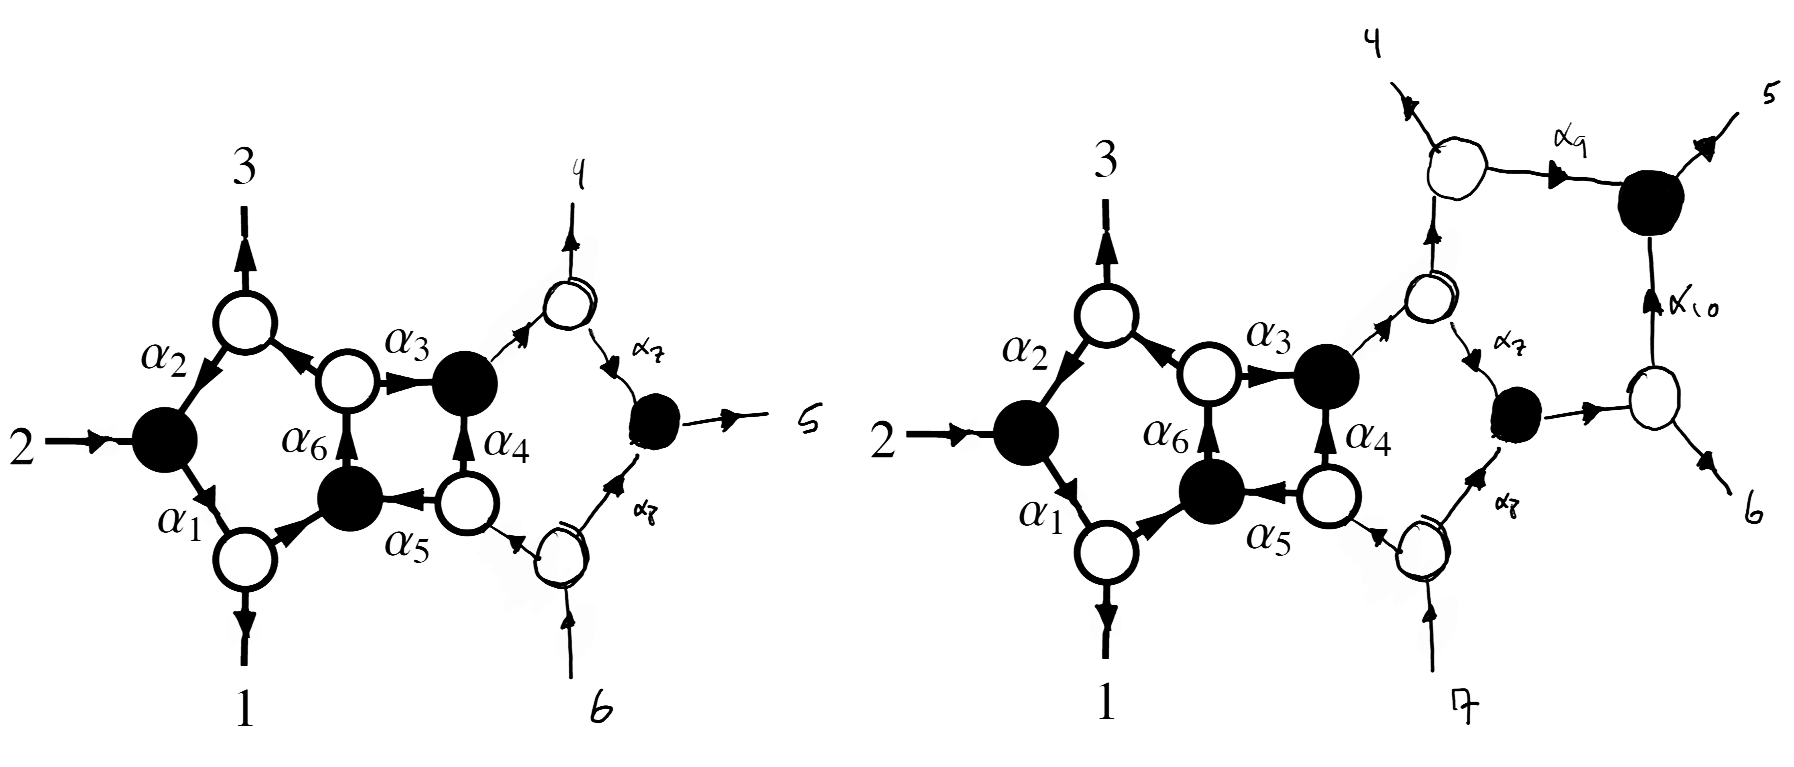
\includegraphics[width=0.7\linewidth]{6+7pt}
	\caption{Six and seven point MHV with cycle}
	\label{fig:two-loop}
\end{figure}
\noindent
The alphas obtained are
\begin{equation}
	\begin{aligned}
		&\text{Six point}:\\
		\alpha_1&=\frac{\ab{13}}{\ab{23}},\,\alpha_2=\frac{\ab{21}}{\ab{13}},\,\alpha_3=\frac{\ab{46}}{\ab{36}},\,\alpha_4=\frac{\ab{34}}{\ab{36}},\\
		\alpha_5&=\frac{\ab{13}}{\ab{36}},\,\alpha_6=\frac{\ab{36}}{\ab{16}},\,\alpha_7=\frac{\ab{56}}{\ab{46}},\,\alpha_8=\frac{\ab{45}}{\ab{46}}.\\
&\text{Seven point}:\\
		\alpha_1&=\frac{\ab{13}}{\ab{23}},\,\alpha_2=\frac{\ab{21}}{\ab{13}},\,\alpha_3=\frac{\ab{47}}{\ab{37}},\,\alpha_4=\frac{\ab{34}}{\ab{37}},\alpha_5=\frac{\ab{13}}{\ab{37}},\\
		\alpha_6&=\frac{\ab{37}}{\ab{17}},\,\alpha_7=\frac{\ab{67}}{\ab{47}},\,\alpha_8=\frac{\ab{46}}{\ab{47}},\,\alpha_9=\frac{\ab{56}}{\ab{46}},\,\alpha_{10}=\frac{\ab{45}}{\ab{46}}.
	\end{aligned}
\end{equation}
The Jacobians from solving the delta functions are
\begin{equation}
	\begin{aligned}
		\text{Six point}:&\\
		&\frac{\ab{13}}{\ab{16}^2\ab{23}^2\ab{36}^2\ab{46}}\\
		\text{Seven point}:&\\
		&\frac{\ab{13}}{\ab{17}^2\ab{23}^2\ab{37}^2\ab{46}\ab{47}}
		\end{aligned}
\end{equation}
with the Jacobian from the cycle being
\begin{equation}
	\begin{aligned}
		\J_6=\frac{\ab{13}\ab{26}}{\ab{16}\ab{23}},~~~~
		\J_7=\frac{\ab{13}\ab{37}}{\ab{17}\ab{23}}
	\end{aligned}
\end{equation}
The forms found by summing over all internal configurations are
\begin{equation}
	\begin{aligned}
		\dd \Omega 
	\end{aligned}
\end{equation}
At eight and nine points we obtain
\begin{figure}[H]
	\centering
	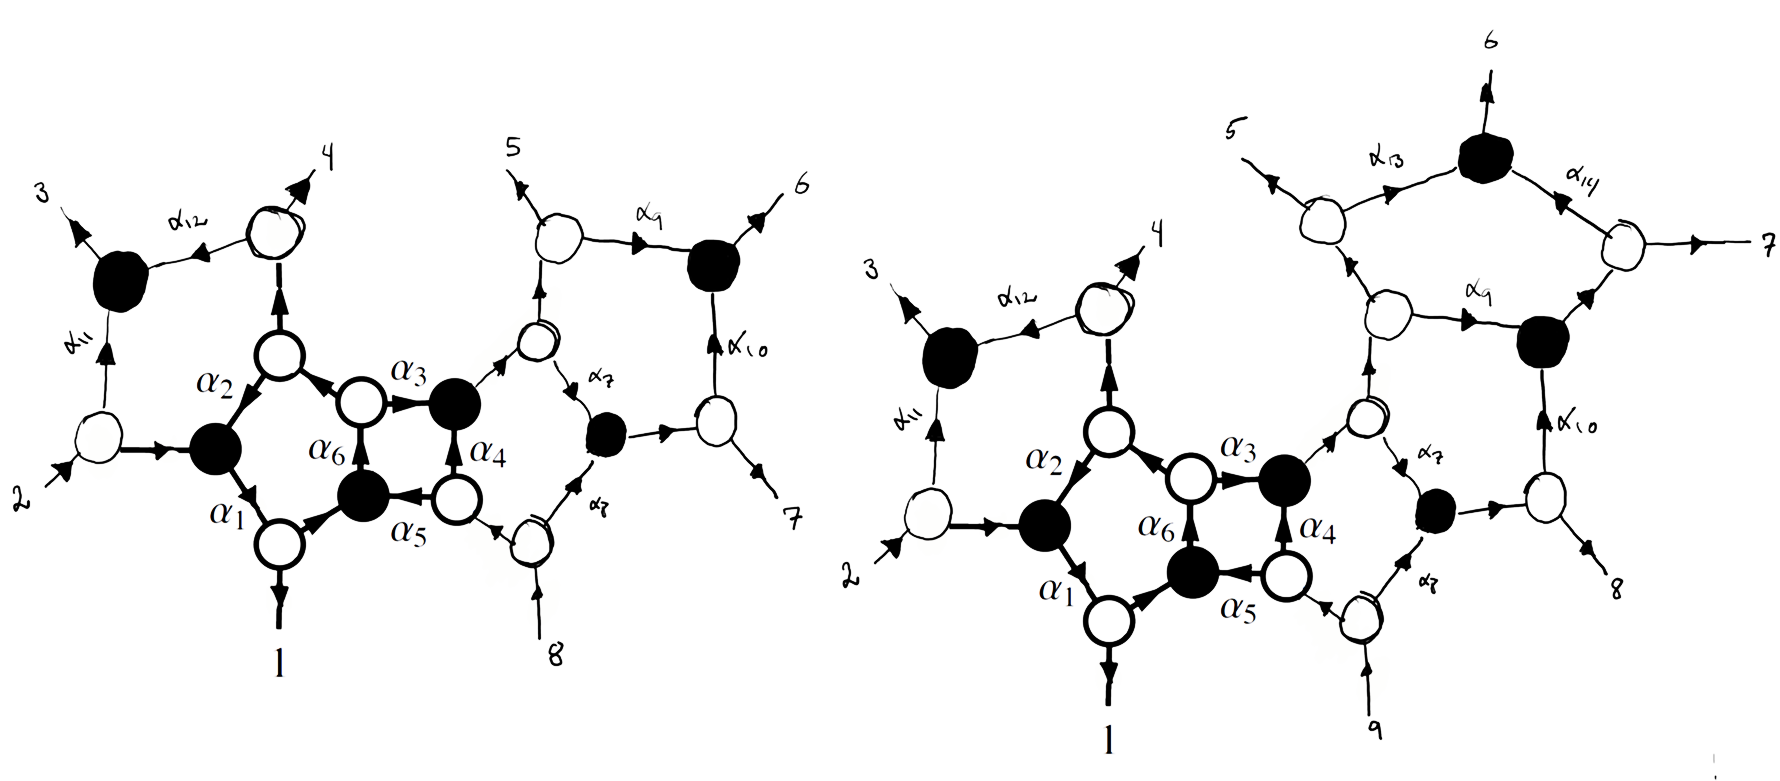
\includegraphics[width=0.7\linewidth]{8+9pt}
	\caption{Eight and nine point MHV with cycle}
	\label{fig:two-loop}
\end{figure}
\noindent
The alphas obtained are
\begin{equation}
	\begin{aligned}
		&\text{Eight point}:\\
	\alpha_1&=\frac{\ab{14}}{\ab{24}},\,\alpha_2=\frac{\ab{21}}{\ab{14}},\,\alpha_3=\frac{\ab{58}}{\ab{48}},\,\alpha_4=\frac{\ab{45}}{\ab{48}},\alpha_5=\frac{\ab{14}}{\ab{48}},\,
	\alpha_6=\frac{\ab{48}}{\ab{18}},\\
	\alpha_7&=\frac{\ab{78}}{\ab{58}},\,\alpha_8=\frac{\ab{57}}{\ab{58}},\,\alpha_9=\frac{\ab{67}}{\ab{57}},\,\alpha_{10}=\frac{\ab{56}}{\ab{57}}
	,\,\alpha_{11}=\frac{\ab{43}}{\ab{24}}
	,\,\alpha_{12}=\frac{\ab{32}}{\ab{24}}
	.\\
		&\text{Nine point}:\\
		\alpha_1&=\frac{\ab{14}}{\ab{24}},\,\alpha_2=\frac{\ab{21}}{\ab{14}},\,\alpha_3=\frac{\ab{59}}{\ab{49}},\,\alpha_4=\frac{\ab{45}}{\ab{49}},\alpha_5=\frac{\ab{14}}{\ab{49}},\,
	\alpha_6=\frac{\ab{49}}{\ab{19}},\,
	\alpha_7=\frac{\ab{89}}{\ab{59}},\\
	\alpha_8&=\frac{\ab{58}}{\ab{59}},\,\alpha_9=\frac{\ab{78}}{\ab{58}},\,\alpha_{10}=\frac{\ab{57}}{\ab{58}}
	,\,\alpha_{11}=\frac{\ab{43}}{\ab{24}}
	,\,\alpha_{12}=\frac{\ab{32}}{\ab{24}}
	,\,\alpha_{13}=\frac{\ab{67}}{\ab{57}}
	,\,\alpha_{14}=\frac{\ab{56}}{\ab{57}}
	.
	\end{aligned}
\end{equation}
The Jacobians from solving the delta functions are
\begin{equation}
	\begin{aligned}
		\text{Eight point}:&\\
		&\frac{\ab{14}}{\ab{18}^2\ab{24}^3\ab{48}^2\ab{57}\ab{58}}\\
		\text{Nine point}:&\\
		&\frac{\ab{14}}{\ab{19}^2\ab{24}^3\ab{49}^2\ab{57}\ab{58}\ab{59}}
	\end{aligned}
\end{equation}
with the Jacobian from the cycle being
\begin{equation}
	\begin{aligned}
		\J_8=\frac{\ab{14}\ab{28}}{\ab{18}\ab{24}},~~~~
		\J_9=\frac{\ab{14}\ab{29}}{\ab{19}\ab{24}}
	\end{aligned}
\end{equation}
\subsection{Higher loops}
We consider
\begin{figure}[H]
	\centering
	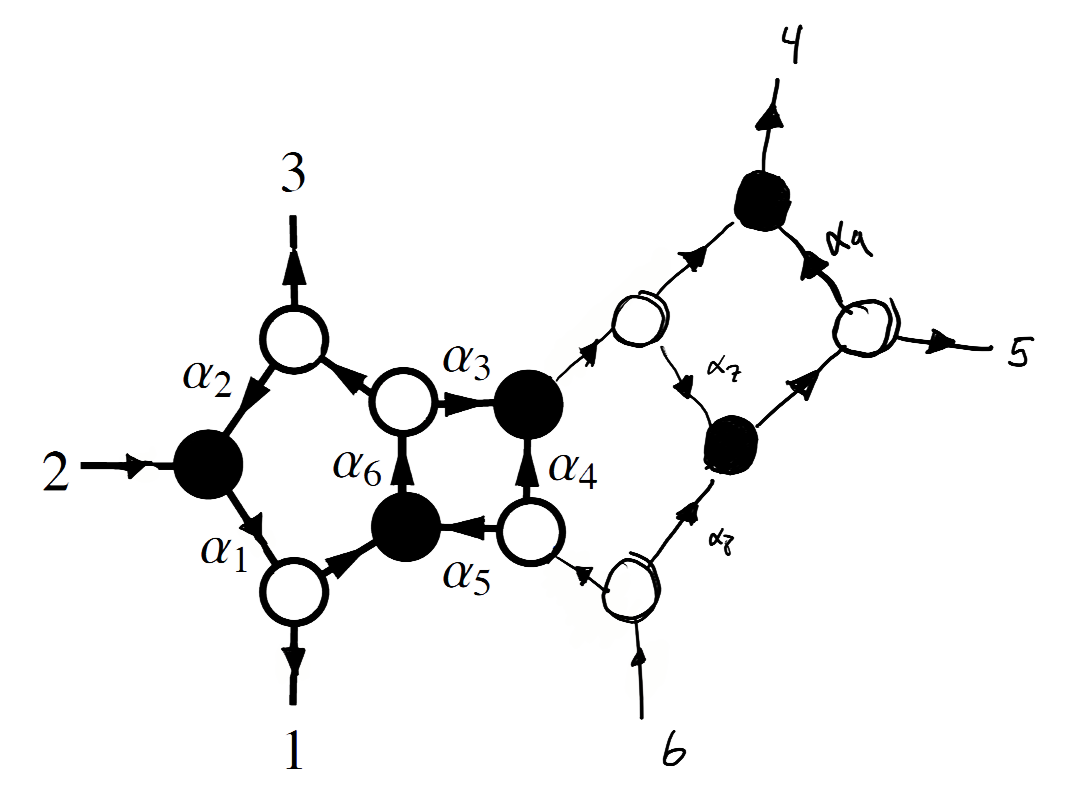
\includegraphics[width=0.4\linewidth]{6pt4l_1}
	\caption{Four-loop six-point MHV with cycle}
	\label{fig:two-loop}
\end{figure}
\noindent
With the following solutions for the edge variables
\begin{equation}
	\begin{aligned}
		\alpha_1&=\frac{\ab{13}}{\ab{23}},\,\alpha_2=\frac{\ab{21}}{13},\,\alpha_3=\frac{\ab{46}-\alpha_9\ab{56}}{\ab{36}}\,\alpha_4=\frac{\ab{34}-\alpha_9\ab{35}}{\ab{36}}\\
		\alpha_5&=\frac{\ab{13}}{\ab{36}},\,\alpha_6=\frac{\ab{36}}{16},\,\alpha_7=\frac{\ab{56}}{\ab{46}-\alpha_9\ab{56}}\,\alpha_8=\frac{\ab{45}}{\ab{46}-\alpha_9\ab{56}}
	\end{aligned}
\end{equation}
The Jacobian in $\mathcal{N}=0$ from solving the delta function is 
\begin{equation}
	\begin{aligned}
		-\frac{\ab{31}\ab{26}^4}{\ab{16}^2\ab{23}^2\ab{36}^2\left(\ab{46}-\alpha_9 \ab{56}\right)}
	\end{aligned}
\end{equation}
while the Jacobian from the cycle is
\begin{equation}
	\begin{aligned}
		\mathcal{J}=\frac{\ab{13}\ab{26}}{\ab{16}\ab{23}}
	\end{aligned}
\end{equation}
The total form summing over all internal configurations is
\begin{equation}
	\begin{aligned}
		\dd\Omega =\frac{\ab{26}^4}{\alpha_9 \ab{12}\ab{23}\ab{45}\ab{56}\ab{61}\left(\alpha_9\ab{45}-\ab{34}\right)}\left(	\left[\frac{\ab{13}\ab{26}}{\ab{16}\ab{23}}\right]^{-4}+
		\left[\frac{\ab{13}\ab{26}}{\ab{12}\ab{36}}\right]^{-4}\right)
	\end{aligned}
\end{equation}
We then treat the following diagram
\begin{figure}[H]
	\centering
	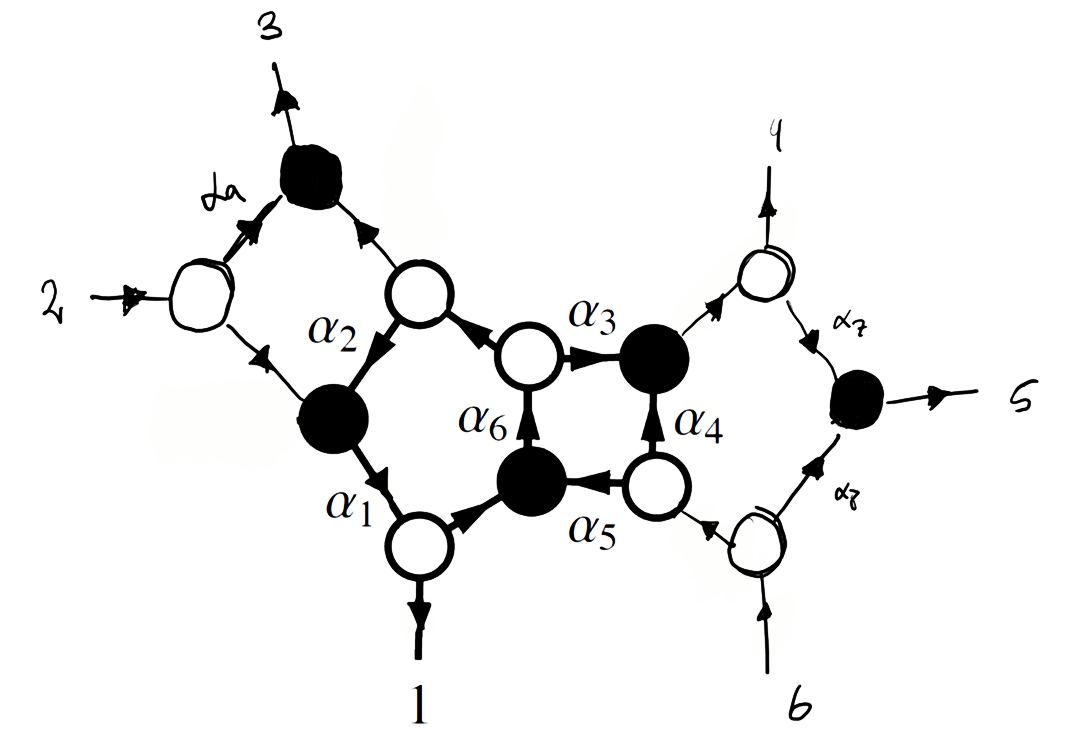
\includegraphics[width=0.4\linewidth]{6pt4l_2}
	\caption{Four-loop six-point MHV with cycle}
	\label{fig:two-loop}
\end{figure}
\noindent
For which we obtain
\begin{equation}
	\begin{aligned}
		\alpha_1&=\frac{\ab{13}-\alpha_9\ab{12}}{\ab{23}},\,\alpha_2=\frac{\ab{21}}{\ab{13}-\alpha_9\ab{12}},\,\alpha_3=\frac{\ab{46}}{\ab{36}-\alpha_9\ab{26}},\,\alpha_4=\frac{\ab{34}-\alpha_9\ab{24}}{\ab{36}-\alpha_9\ab{26}}\\
		\alpha_5&=\frac{\ab{13}-\alpha_9\ab{12}}{\ab{36}-\alpha_9\ab{26}},\,\alpha_6=\frac{\ab{36}-\alpha_9\ab{26}}{16},\,\alpha_7=\frac{\ab{56}}{\ab{46}}\,\alpha_8=\frac{\ab{45}}{\ab{46}}
	\end{aligned}
\end{equation}
The Jacobian in $\mathcal{N}=0$ from solving the delta function is 
\begin{equation}
	\begin{aligned}
		\frac{\left(\alpha_9\ab{12}-\ab{31}\right)\ab{26}^4}{\ab{16}^2\ab{23}^2\ab{46}\left(\ab{36}-\alpha_9 \ab{26}\right)^2}
	\end{aligned}
\end{equation}
while the Jacobian from the cycle is
\begin{equation}
	\begin{aligned}
		\mathcal{J}=\frac{\ab{26}\left(\ab{13}-\alpha_9\ab{12}\right)}{\ab{16}\ab{23}}
	\end{aligned}
\end{equation}
The total form summing over all internal configurations is
\begin{equation}
	\begin{aligned}
		\dd\Omega =\frac{\ab{26}^4}{\alpha_9 \ab{12}\ab{23}\ab{45}\ab{56}\ab{61}\left(\alpha_9\ab{24}-\ab{34}\right)}\left(	\left[\frac{\ab{26}\left(\ab{13}-\alpha_9\ab{12}\right)}{\ab{16}\ab{23}}\right]^{-4}+
		\left[\frac{\ab{26}\left(\ab{13}-\alpha_9\ab{12}\right)}{\ab{12}\left(\ab{36}-\alpha_9\ab{26}\right)}\right]^{-4}\right)
	\end{aligned}
\end{equation}
%%%%%%%%%%%%%%%%%%%%%%%%%%%%%%
%%%%%%%%%%%%%%%%%%%%%%%%%%%%%%
%%%%%%%%%%%%%%%%%%%%%%%%%%%%%%
%%%%%%%%%%%%%%%%%%%%%%%%%%%%%%
%%%%%%%%%%%%%%%%%%%%%%%%%%%%%%
%%%%%%%%%%%%%%%%%%%%%%%%%%%%%%
%%%%%%%%%%%%%%%%%%%%%%%%%%%%%%
%%%%%%%%%%%%%%%%%%%%%%%%%%%%%%
%%%%%%%%%%%%%%%%%%%%%%%%%%%%%%
\newpage
\begin{thebibliography}{99}
%\cite{Arkani-Hamed:2010zjl}
\bibitem{amp1}
N.~Arkani-Hamed, J.~L.~Bourjaily, F.~Cachazo, S.~Caron-Huot and J.~Trnka,
%``The All-Loop Integrand For Scattering Amplitudes in Planar N=4 SYM,''
JHEP \textbf{01}, 041 (2011)
doi:10.1007/JHEP01(2011)041
[arXiv:1008.2958 [hep-th]].
%411 citations counted in INSPIRE as of 10 Oct 2021
%\cite{Elvang:2015rqa}
\bibitem{Elvang}
H.~Elvang and Y.~t.~Huang,
``Scattering Amplitudes in Gauge Theory and Gravity,''
%18 citations counted in INSPIRE as of 10 Oct 2021
%\cite{Arkani-Hamed:2012zlh}
%393 citations counted in INSPIRE as of 10 Oct 2021
%\cite{Arkani-Hamed:2013jha}
\bibitem{amp3}
N.~Arkani-Hamed and J.~Trnka,
%``The Amplituhedron,''
JHEP \textbf{10}, 030 (2014)
doi:10.1007/JHEP10(2014)030
[arXiv:1312.2007 [hep-th]].
%352 citations counted in INSPIRE as of 10 Oct 2021
%\cite{Arkani-Hamed:2013kca}
\bibitem{amp4}
N.~Arkani-Hamed and J.~Trnka,
%``Into the Amplituhedron,''
JHEP \textbf{12}, 182 (2014)
doi:10.1007/JHEP12(2014)182
[arXiv:1312.7878 [hep-th]].
%133 citations counted in INSPIRE as of 10 Oct 2021
\bibitem{amp6}
N.~Arkani-Hamed, A.~Hodges and J.~Trnka,
%``Positive Amplitudes In The Amplituhedron,''
JHEP \textbf{08}, 030 (2015)
doi:10.1007/JHEP08(2015)030
[arXiv:1412.8478 [hep-th]].
%70 citations counted in INSPIRE as of 10 Oct 2021
\bibitem{on1}
N.~Arkani-Hamed, J.~L.~Bourjaily, F.~Cachazo, A.~Postnikov and J.~Trnka,
%``On-Shell Structures of MHV Amplitudes Beyond the Planar Limit,''
JHEP \textbf{06}, 179 (2015)
doi:10.1007/JHEP06(2015)179
[arXiv:1412.8475 [hep-th]].
%68 citations counted in INSPIRE as of 10 Oct 2021
%\cite{Herrmann:2016qea}
\bibitem{amp2}
N.~Arkani-Hamed, J.~L.~Bourjaily, F.~Cachazo, A.~B.~Goncharov, A.~Postnikov and J.~Trnka,
%``Grassmannian Geometry of Scattering Amplitudes,''
doi:10.1017/CBO9781316091548
[arXiv:1212.5605 [hep-th]].
\bibitem{on2}
E.~Herrmann and J.~Trnka,
%``Gravity On-shell Diagrams,''
JHEP \textbf{11}, 136 (2016)
doi:10.1007/JHEP11(2016)136
[arXiv:1604.03479 [hep-th]].
%42 citations counted in INSPIRE as of 10 Oct 2021
%\fi
\end{thebibliography}
\end{document}

